%&latex
\documentclass[12pt]{article}
\usepackage{amsmath,amsfonts}
\usepackage{graphicx,psfrag,epsf}
\usepackage{enumerate}
\usepackage{natbib}
\usepackage{url} % not crucial - just used below for the URL 
\usepackage{etoolbox}

%\pdfminorversion=4
% NOTE: To produce blinded version, replace "0" with "1" below.
\newcommand{\blind}{0}

% DON'T change margins - should be 1 inch all around.
\addtolength{\oddsidemargin}{-.5in}%
\addtolength{\evensidemargin}{-.5in}%
\addtolength{\textwidth}{1in}%
\addtolength{\textheight}{-.3in}%
\addtolength{\topmargin}{-.8in}%
\graphicspath{{figures_tables/}}


\begin{document}
\newtoggle{thesis}
\togglefalse{thesis}
% \bibliographystyle{natbib}

\def\spacingset#1{\renewcommand{\baselinestretch}%
{#1}\small\normalsize} \spacingset{1}


%%%%%%%%%%%%%%%%%%%%%%%%%%%%%%%%%%%%%%%%%%%%%%%%%%%%%%%%%%%%%%%%%%%%%%%%%%%%%%

\if1\blind
{
  \title{\bf A nonparametric Bayesian analysis of RNA-seq gene expression data}
  \author{Author 1\thanks{
    The author gratefully acknowledges Dr. Jarad Niemi for advise and comments.\textit{This project was funded in part by a grant from the NIH, XXXX.}}\hspace{.2cm}\\
    Department of Statistics, Iowa State University}
  \maketitle
} \fi

\if0\blind
{
  \bigskip
  \bigskip
  \bigskip
  \begin{center}
    {\LARGE\bf A nonparametric Bayesian analysis of RNA-seq gene expression data}
\end{center}
  \medskip
} \fi

\bigskip
\begin{abstract}
The text of your abstract. 200 or fewer words.
\end{abstract}

\noindent%
{\it Keywords:}  3 to 6 keywords, that do not appear in the title
\vfill

\newpage
\tableofcontents

\spacingset{1.45} % DON'T change the spacing!

\section{Introduction}
Heterosis, or hybrid vigor, refers to biological differences seen in offspring of two inbred parents, which give the hybrid qualities superior to either parent. While the phenomenon is well-known and widely exploited, its causes at the molecular level are not well understood \citep{paschold}. New technologies that can simultaneously measure the expression of tens of thousands of genes provide an opportunity to shed light on these mechanisms.

Recently, RNA-seq technology has supplanted microarrays as the primary platform for these studies \citep{wang2009rna}. Statistical methods to analyze RNA-seq data have proliferated \citep{voom,deseq2014,mccarthy,liu,landau}. Because cost limits the number of samples that can be sequenced, the identification of interesting genes in gene expression profiling studies falls into the ``$n \ll p$" paradigm. In this paradigm, noise in the data tends to dominate the signal. Various statistical methods have been developed to mitigate this problem. One general approach is to hierarchical modeling.

Hierarchical, or multi-level, models provide a mechanism to borrow strength across groups present in the data by learning the underlying distribution of the first-level model parameters. The case for using hierarchical models for RNA-seq data is compelling because there are a large number of genes, potentially providing substantial information about the distribution of gene-specific parameters, as well as a strong incentive to borrow information since there are often few samples with which to estimate any given gene-specific parameter. \citet{niemi} observed that the choice of parametric family for the hierarchical model impacts both estimation and the ranking of genes. It seems that appropriate modeling of the underlying distribution of the gene-specific parameters will lead to better results. To avoid misspecification of the distribution of gene-specific parameters, one might choose to model them nonparametrically; for example, \citet{liu} proposed a semiparametric model for differential expression. In their model, the parameter representing the mean log-fold-change between the two treatments was modeled with a Dirichlet process (DP).

RNA-seq allows for direct mapping of reads to genetic features, so measurements are counts of total reads. While most RNA-seq methods we have seen use the negative binomial (NB) distribution \citet{mccarthy} provided a theoretical motivation for directly modeling the counts via a Poisson mixture, \citet{voom} demonstrated a method for estimating precision weights, making a normal data model a viable alternative to count-based methods. We choose to take advantage of the normal model, which allows us to exploit conditional conjugacy work with lower-dimensional sufficient statistics. This eases the computation burden, which can be a considerable benefit when conducting fully Bayesian inference.
%
% R A common element of such methods is the regularization of gene-specific analysis to decrease false detection rates and improve estimation accuracy.
%Because the presence of a meaningful biological effect fits awkwardly into the framework, we approach the problem of  addressed through estimation \citet{deseq2014}. This is the approach that we pursue here.

% Current estimation methodologies can be understood as improving upon a ``straight" estimator by modeling gene-specific model parameters to borrow information across genes. \textit{Insert analogy to Stein's estimator}.


% The advantages of such hierarchical models have been shown to work well in practice, regardless of whether the distributional form of the random effects restrict should be assumed to have a simple form, will tend to be estimated very precisely. If the model is overly simplistic, the information borrowed across genes will tend to be quite vague.

% A rationale for hierarchical modeling in gene expression is to regularize estimation for gene-specific parameters by shrinking the posterior distribution of these parameters toward the mass of their distribution. Due to their faster computational speed, empirical Bayes methods have been preferred by practitioners to fully Bayesian methods. One argument for their use is that when $G$ is large, $\mathcal{P}$ should be have low variance in the posterior, so that inference based on an estimate of $\mathcal{P}$ should be quite similar to a fully Bayesian analysis which integrates over the uncertainty in $\mathcal{P}$. \citet{landau2016high} ran a series of simulation studies lending support to this claim for a class of hierarchical models.
%
% Whether the method used is empirical Bayes or fully Bayesian, the use of hierarchical models in this area has led to improvements in estimation and testing. \citet{niemi} observed that the choice of parametric family can impact both estimation and the ranking of genes. It seems that appropriate modeling of the underlying distribution of the gene-specific parameters will lead to better results; in contrast, misspecification of the distribution will limit both the accuracy and precision that can be obtained in estimation of the parameters.
%The theory which supports these arguments assumes that the complexity of $\mathcal{P}$ can be described by a fixed number of parameters.
%Whether or not a suitable, parsimonious parameteric model can be found for the gene-specific parameters in gene expression data is a question that
% Indeed, many `shrinkage priors', or equivalent methods, has proven to be a useful tool even when the distributional form is misspecified.

% Because of its essential role, the shape of the tail, vis a vis the choice of the hierarchical model, should be considered. We showed that the choice affected the number of genes called as well as which ones.
%
% Several interesting approaches to improving the hierarchical model have been considered. \citet*{lithio} considered reparameterizing the linear predictors to minimize the correlations of the gene-specific effects, in part to motivate the use of independent prior distributions. They find that the parameterization has a significant impact on the performance of the model.
% %We hope avoid such sensitivities by using nonparametric prior distributions for these parameters.
% \citet{voom} proposed a method which unlocks linear modeling of RNA-seq data by estimating precision weights for each RNA-seq count. This is accomplished by estimating the mean variance relationship parametrically by fitting a loess curve using independent estimates by gene of the average log expression and fourth root of the error variance. This between-gene information is then applied within genes via precision weights. \citet{liu} proposed a semiparametric model for differential expression. In their model, a gamma mixture of Poisson was used and information was borrowed across genes only for the log-fold-change parameter, which was given a Dirichlet process prior.
% 
The road map for this paper is as follows: In Section~\ref{sec:data}, we describe the heterosis data of \citet{paschold}. Next, in Section~\ref{sec:model}, we first motivate the use of Bayesian nonparametric models, using an example to illustrate the consequences of misspecification in hierarchical models as well benefits of using a flexible DP prior. We then propose a Bayesian nonparametric model that extends the approach taken in \citet{liu} by modeling all gene-specific parameters with a DP. After specifying the model, we describe our implementation including data steps prior to modeling. Section~\ref{sec:ss1} describes a simulation study comparing detection of heterosis and point estimates obtained from our model to those obtained using a non-hierarchical approach but that uses the same data normalization and precision weighting. In Section~\ref{sec:ss2} we present a second simulation study, also focused on detection of heterosis and parameter estimation, that compares performance of our method to two popular negative-binomial based methods, \texttt{DESeq2} and \texttt{edgeR} \citep{edger2010, deseq2014}. Next, in Section~\ref{analysis} we present results for the Paschold data set and contrast them with those from the original paper \cite{paschold} and with those obtained by \citet{landau} who used an independent parametric model for the gene-specific parameters.
% \citet{landau-compute} implemented a Gibbs sampler for a parametric Bayesian hierarchical model for RNA-seq data using a graphics processing unit (GPU) to accelerate computation. Their work helped to inspired this Bayesian nonparametric approach.


\section{RNA-seq gene expression data}
\label{sec:data}
The starting point for our analyses is an array of RNA-seq total aligned read counts measuring the abundance of a particular messenger RNA transcript in a sample. Such an array consists of $G$ rows and $N$ columns, corresponding to genes and samples, respectively. The abundance of a transcript is often referred to as gene expression; we will follow this convention here. For more details on data collection and preprocessing of RNA-seq data, please see \citet{datta2014}.

A simple analysis of RNA-seq data may be achieved by analyzing each gene independently. The experimental design can generally considered the same for all genes. Select rows for an example data set are shown below in Table \ref{counts}.

% latex table generated in R 3.4.2 by xtable 1.8-2 package
% Thu Nov 09 17:08:22 2017
% latex table generated in R 3.4.2 by xtable 1.8-2 package
% Thu Nov 09 17:12:54 2017
\begin{table}[ht]
\centering
\begin{minipage}{.8\textwidth}
\caption{\small Selected rows from RNA-seq data set showing total aligned read counts for selected genes. Columns are grouped by genotype. Exemplar genes for different types of heterosis are shown.}
\label{counts}
\end{minipage}
\\[.25cm]
\scalebox{0.6}{
\begin{tabular}{cl|rrrr|rrrr|rrrr|rrrr}
  \toprule
GeneID & \multicolumn{1}{c}{type of heterosis} &  \multicolumn{4}{c}{B73} & \multicolumn{4}{c}{B73xMo17} & \multicolumn{4}{c}{Mo17xB73}& \multicolumn{4}{c}{Mo17}  \\
  \midrule
GRMZM2G306345 & HPH & 1431 & 1199 & 1235 & 1569 & 2055 & 1652 & 2149 & 2168 & 2415 & 1815 & 2142 & 2369 & 1127 & 987 & 1672 & 1518 \\
GRMZM2G149543 &  LPH &  86 &  62 & 131 & 128 &  52 &  43 &  85 &  95 &  60 &  23 &  63 &  74 &  85 &  71 & 178 & 205 \\
GRMZM2G079613 &  mixed & 122 &  98 & 146 & 150 &  73 &  77 & 159 & 127 & 178 & 122 & 259 & 252 & 108 & 103 & 207 & 171 \\
AC194005.3\_FG004 &  neither &  30 &  31 &  42 &  48 &  17 &  15 &  22 &  26 &  16 &  13 &  16 &  22 &   2 &   2 &   2 &   2 \\
   \bottomrule
\end{tabular}
}
\end{table}
% 
\subsection{Maize data of Paschold et al.}
\label{intro-paschold}
The data come from \cite{paschold}. We work with the count of total aligned reads for two parental lines, B73 and Mo17, and the reciprocal hybrid genotypes, B73$\times$Mo17 and Mo17$\times$B73, for 39,656 genes. Of these, we exclude 2835 genes where all counts were exactly zero. Each genotype had 4 biological replicates, each produced from primary roots of 10 kernels 3.5 days after germination. Sequencing of the 16 samples was done using Illumina methodology and equipment in 1 run using 2 flowcells. Reads were mapped to the whole reference genome using the short reads aligner, NOVOALIGN. For more specifics, please see \cite{paschold}.

% Heterosis refers to the phenomenon whereby, a hybrid type, that is a genotype which a cross of two inbred parental genotypes, exhibits some phenotypic advantage over either of the two parents. Often this is of practical importance in agriculture, where great effort and expense has be invested in identifying and breeding new varieties, often to increase productivity, quality or disease resistance. While the effects of heterosis are quite well-known, the genetic causes are not clear. Hopefully, new sequencing technologies, with the help of good statistical methods, will help researchers understand the mechanisms underlying heterosis to help efforts to improve agriculture, making it more efficient and productive.

% The most interesting and useful form of heterosis, known as hybrid vigor, occurs when hybrid progeny display a mean phenotype that is superior to  both parental phenotypic means.  This heterosis phenomenon was scientifically documented in plants by \cite{darwin1876effects} and has long been used to improve agricultural production. One classic example involves hybrid maize offspring that are taller, faster to mature, and yield considerably more grain than their inbred parents \citep{hallauer1981quantitative, hallauer2010quantitative}.
\begin{figure}
\centering
\begin{minipage}{.8\textwidth}
\includegraphics[width=\textwidth]{count_dist_by_sample}
\caption{Distribution of total read counts plus 1 by sample, grouped by genotype, for all 16 RNA-seq samples in the maize data.}
\label{fig:count-dist}
\end{minipage}
\end{figure}

The counts range in value from 0 to 38,006 with a mean value of 255.5 and a median value of 37. Figure \ref{fig:count-dist} shows the distribution of the total read counts plus 1 by sample. While the distributions look fairly consistent across samples, there are some differences in the lower quartiles. The replicate numbers on the x-axis can be used to identify the flow cell; replicates 1 and 2 were sequenced in flow cell 1, while replicates 3 and 4 were sequenced in flow cell 2. The differences between the flow cells shown in the lower quartile of the boxplots for the hybrids suggest that flow cell 1 was more thoroughly sequenced than flowcell 2.


To identify genes which are likely to play a role in heterosis, we look for genes where the ordering of the average expression levels for the 4 genotypes exhibits one of several patterns. We say a gene expresses heterosis, when the expected value of a hybrid genotype differs from the average of the expected values of the two parents. To be precise, we define multiple kinds of heterosis in terms of the mean expression levels of the genotypes. High-parent heterosis (HPH) occurs when the expected value of a hybrid is higher than that of both parents. Similarly, low-parent heterosis (LPH) occurs when the expected value of a hybrid is lower than that of both parents. The first two genes (rows) in Table \ref{counts} are exemplar genes of HPH and LPH, respectively. The third gene appears that B73$\times$Mo17 displays LPH while Mo17$\times$B73 displays HPH, and in the last gene the hybrid expression appears to lie between that of the parents. Here too, we see the apparent flow cell effects, since within a genotype there appear to be consistent differences between the first and second pairs of replicates.

\section{Bayesian nonparametric model}
The advantage of hierarchical modeling generally is that that by assumming a distribution on some model parameters, we can improve inference by borrowing information, i.e. allowing data which doesn't have a direct dependence on a parameter to inform indirectly about the parameter through the parameter's distribution. Misspecification of the form of that hierarchical distribution can lead to incorrect borrowing of information. In practice, this issue is often overlooked. One reason for this is that in many cases it is difficult to check whether the hierarchical distribution is misspecified. Another reason is that there can be utility to using a hierarchical model, even when the hierarchical distribution is misspecified.

\subsection{Illustration}
\label{subsec:illustration}
To provide an example of the ideas in the preceding paragraph and to motivate the development of our model, we given the following example. 
% Let $y_{gn},\; g=1,\ldots,200,\;n=1,2,3$, and suppose we are interested in hypotheses concerning $\op{E}(y_{gn})=\mu_g$. Suppose further that we can reasonably assume that $y_{gn}|\mu_g \ind \op{N}(\mu_g,\sigma^2)$, i.e. the data are conditionally normal with unknown means and unknown constant error variance. 
We simulate data as follows, $\mu_g \ind 1/3\op{N}(-4,1)+1/3\op{N}(0,1)+1/3\op{N}(4,1)$. Conditional on $\mu$, we simulate $y_{gn}|\mu_g \ind \op{N}(\mu_g,\sigma^2=2^2),\; g=1,\ldots,200,\;n=1,2,3$. Now, suppose we observe $y$ and assume the (true) data model, but $\mu_g$ and the common error variance, $\sigma^2$, are all unknown. A histogram of the sample means, $\hat{\mu}_g$ is shown in the top panel of Figure~\ref{predictive}. Next, we fit three Bayesian models to the data.
\begin{enumerate}
\item Normal model: $\mu_g \ind \op{N}(\eta, \tau^2)$, with diffuse proper priors on $\eta$ and $\tau^2$
\item Correct model: $\mu_g \sim \pi_1\op{N}(\eta_1,\tau^2)+\pi_2\op{N}(\eta_2,\tau^2)+\pi_3\op{N}(\eta_3,\tau^2)$, also with diffuse proper priors on $\eta_j$ and $\tau^2$ and a $\op{Dir}(1,1,1)$ prior on $\pi$
\item DP model: $\mu_g \ind \mathcal{P}$ with $\mathcal{P} \sim \op{DP}\left(\alpha \op{N}(0,5^2)\right)$ and an informative prior on $\alpha$
\end{enumerate}. 

Critically, this last model allows us to be agnostic about the modality of $\mathcal{P}$; further details are given in the next section.

\begin{figure}[ht]
\centering
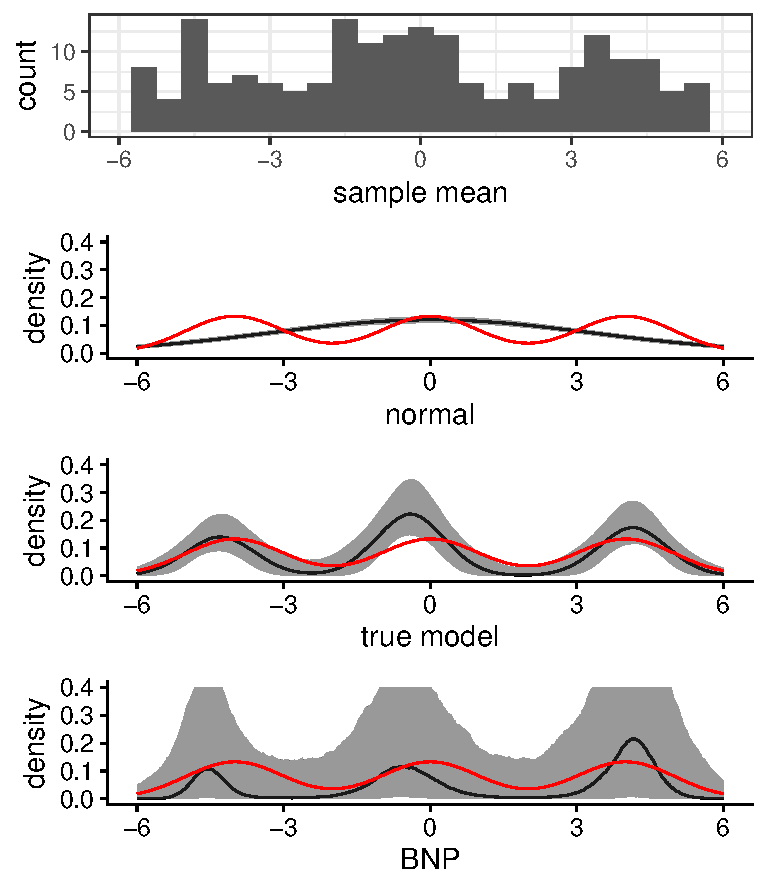
\includegraphics[width=.5\textwidth]{toy_ex/predictive}
\begin{minipage}{.8\textwidth}
\caption{\small Top: Sample averages for the simulated trimodal data. The next three rows correspond to pointwise posterior estimates and 90\% credible intervals for the predictive density for a new $\mu_g$. For the DP model, a weighted kernel density estimate employing a bandwidth of 0.1  was used for each posterior draws of $\mathcal{P}$, as the posterior draws do not have a density with respect to Lebesgue measure.}
\label{predictive}
\end{minipage}
\end{figure}


The bottom three panels of Figure \ref{predictive} show density estimates and 90\% pointwise credible intervals for the predictive distributions for a new $\mu_g$ based on the posteriors the three models. For the Normal model and the Correct model, these were computed by taking quantiles of the sampled density evaluated on a grid. For the DP model, the sample density was estimated using a weighted kernel with bandwidth of 0.1 because samples of $\mathcal{P}$ do not have a density with respect to Lebesgue measure. The true generating model for the $\mu_g$ is shown in red. The posterior for the density of $\mu_g$ under the normal model has less uncertainty but is concentrated around an incorrect answer because of its inflexibility. Both the Correct and the DP models contain much of the true density within the pointwise uncertainty intervals. The DP model shows a great deal more posterior uncertainty because it does not assume a parametric model for $\mu_g$. Despite the increased uncertainty in the predictive distribution, the posterior estimation under the DP model is nearly as good as it is under the true model; the left panel of Figure~\ref{precision} shows the lengths of the posterior 95\% credible intervals for the $\mu_g$ sorted by their length for the three models; the dotted lines represent correspond to a non-hierarchical analysis (independent, uniform priors on $\mu_g$) with $\sigma^2$ known ($+/- 4/\sqrt{3}$). For this data set, we see that both the nonparametric and true models have less posterior uncertainty than the normal model on average, while all three hierarchical models have substantially less uncertainty than a non-hierarchical model. The right panel shows histograms of the gene specific RMSE, $[\int (\mu_g - \mu_{g0})^2 p(\mu_g|y) d\mu_g]^{1/2}$, computed for each $g$ under the three models, where $\mu_{g0}$ is the true value. Again, we see that estimation is substantially improved when the hierarchical distribution is modelled appropriately.

% \begin{figure}[h!]
% 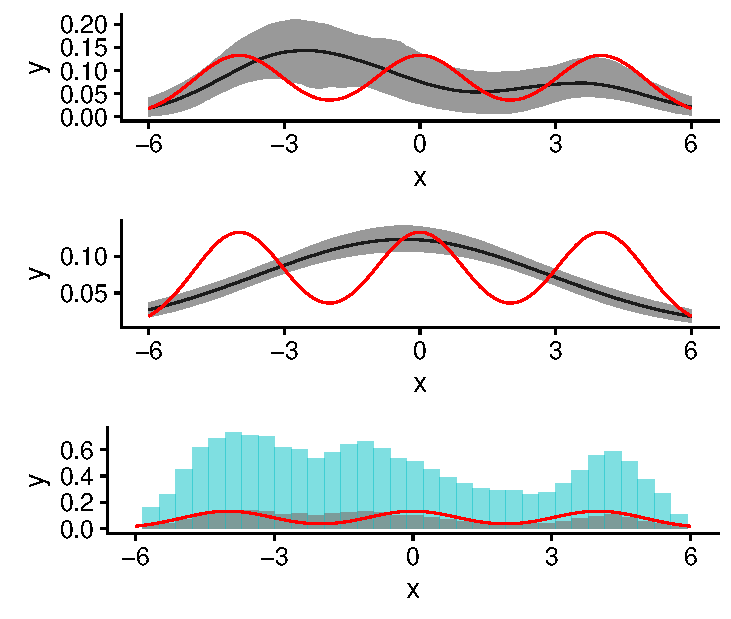
\includegraphics[width=.5\textwidth]{toy_ex/post-pred}
% \caption{Pointwise density estimates for three posterior models based on simulated data of Subsection~\ref{subsec:illustration}}
% \label{ex-predictive}
% \end{figure}

\begin{figure}[h!]
\centering
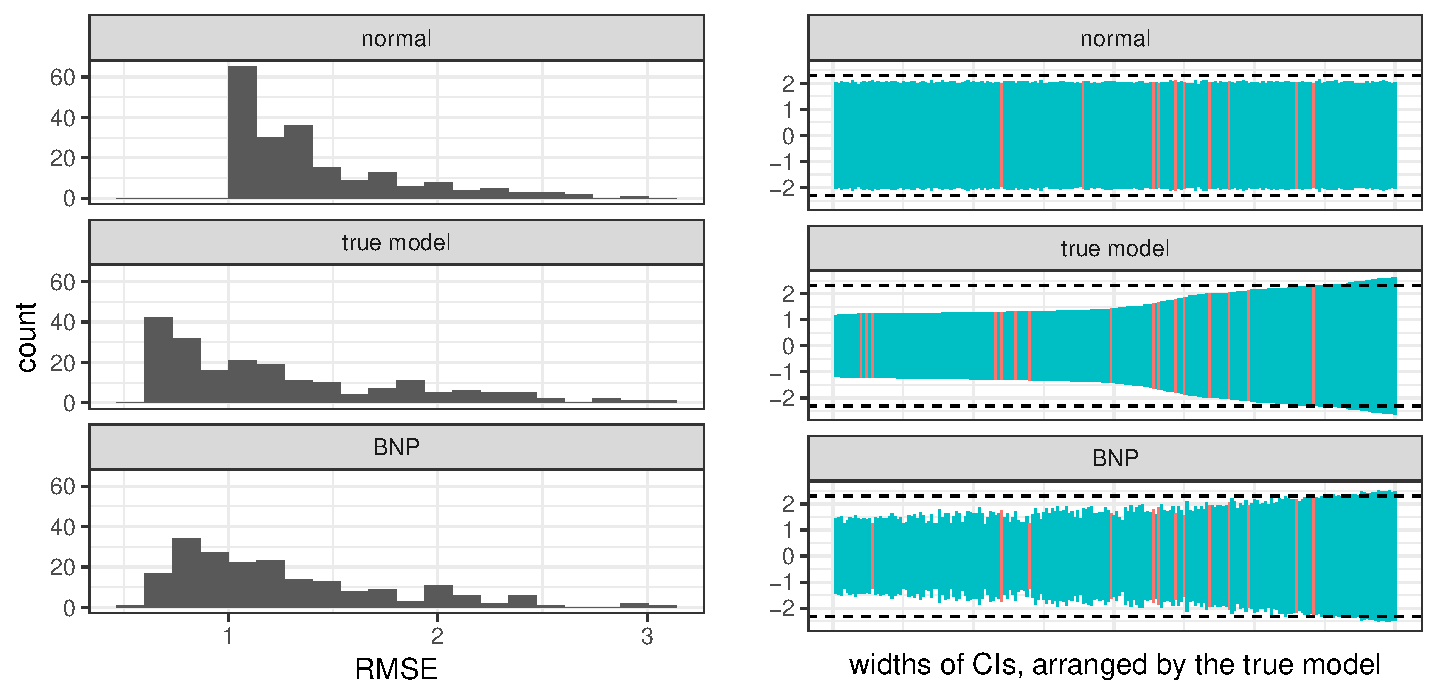
\includegraphics[width=\textwidth]{toy_ex/precision}
\begin{minipage}{.8\textwidth}
\caption{\small Left: Histograms of gene specific RMSE based on posteriors for these models. Right: The widths of the 95\% posterior credible intervals for $\mu_g$ under the three hierarchical models, arranged by the width for the true model. Intervals which failed to cover the true value are colored red. The dashed lines correspond approximately to credible intervals with independent uniform priors on $\mu_g$.}
\label{precision}
\end{minipage}
\end{figure}


\subsection{BNP model for RNA-seq data}
\label{sec:model}
Let $y_{gn}$ represent the normalized log-cpm for gene $g$, sample $n$ and let X be the model matrix. Let $x_{n}^\top$ be the row of a model matrix corresponding to sample $n$. Let $g=1,...,G$ and $n=1,...N$ index genes and samples, respectively. We model
\begin{equation}
y_{gn} \sim \op{N} \left( x_{n}^\top \beta_g, \frac{\sigma^2_g}{w_{gn}} \right)
\end{equation}
where $w_{gn}$ is a given relative precision for $y_{gn}$. While not critical to our method, the inclusion of these precisions allows us to avoid dependence on the assumption of constant variance within genes. This is discussed further in Section \ref{norm-weight}. As discussed in the previous Section, we intend to model the gene-specific parameters nonparametrically, letting the vector of gene specific parameters follow a Dirichlet process. This is denoted by
\begin{equation}
\left(\beta_g^\top,\sigma^2_g\right) \ind \mathcal{P},\quad \mathcal{P} \sim \op{DP}(\alpha \mbox{Q}),
\end{equation}
where $\op{DP}(\alpha \mbox{Q})$ is a Dirichlet process with concentration parameter, $\alpha$, and base distribution $\mbox{Q}$.

The DP satisfies two requirements proposed by \citet{ferguson} for priors over probability distributions, that it have large support on the space of probability distributions and that it be computationally tractable \citep{ferguson}. The tractibility of the DP is important, because it makes inference computationally feasible. The large support allows us to discard unwarranted parametric assumptions about $\mathcal{P}$.

The stick-breaking characterization of the DP, due to \citet{sethuraman}, says that 
\begin{equation}
\label{dp-def}
\mathcal{P} =\sum_{k=1}^\infty \pi_k \delta_{\left(\tilde{\beta}_k^\top ,\tilde{\sigma}^2_k\right)},\quad \pi_k = \nu_k \prod_{l<k}(1-\nu_l), \quad 
\nu_k \ind \op{Beta}(1, \alpha),\; \alpha>0,
\end{equation}
where $\left(\tilde{\beta}_k^\top ,\tilde{\sigma}^2_k\right) \ind Q$, and where $\delta_{x}$ represents the Dirac delta function. It is clear from Sethuraman's representation of the DP that $\mathcal{P}$ is almost surely discrete. The name, ``stick-breaking", given to this characterization, is illuminated by noting the specification of the cluster weights, $\pi_k$, in terms of the independent $\nu_k$ can be rewritten as
\begin{equation}
\label{eq:pi}
\pi_k = \nu_k\left(1-\sum_{l<k}\pi_l\right),
\end{equation} so $\nu_k$ has the interpretation of the relative size of $\pi_k$ as compared to the remaining ``stick", $1-\sum_{l<k}$.

A consequence of (\ref{dp-def}) is that $\op{E}(\pi_k)<\op{E}(\pi_l),\;k>l$ and that $E(\pi_k)=\left[1/(\alpha+1\right]\left[\alpha/(\alpha+1)\right]^{k-1} = \alpha \left[\alpha/(\alpha+1)\right]^{k}$, which tell us that $\pi_k$ decreases in expectation in $k$, is decreasing quickly for small values of $\alpha$ and slowly for large values. It is important to understand that this model gives positive prior probability that $(\beta_g^\top,\sigma_g^2)=(\beta_{g'}^\top,\sigma_{g'}^2)$ for any $g$ and $g'$. Another related fact involving $\alpha$, pointed out by \citet{antoniak}, is that the expected number of unique values of $(\beta_g^\top,\sigma^2_g)$ is 
\begin{equation}
\label{exp-num-clust}
\sum_{i=1}^G \frac{\alpha}{\alpha + i - 1}.
\end{equation}  The bet made on sparsity by assuming this latent clustering allows for such flexibility in learning $\mathcal{P}$, without overfitting the model to the data.

Equation (\ref{eq:pi}) suggests that for large $K$, $\pi_\ell$ are negligible for $\ell>K$. We use this fact to justify our use of a truncated approximation to (\ref{dp-def}),
\begin{equation}
\label{trunc-dp-def}
\mathcal{P} =\sum_{k=1}^K \pi_k \delta_{\left(\tilde{\beta}_k^\top ,\tilde{\sigma}^2_k\right)},\quad \pi_k = \nu_k \prod_{l<k}(1-\nu_l), \quad 
\nu_k \ind \op{Beta}(1, \alpha),\; \alpha>0,\; k<K,\; \nu_K:=1.
\end{equation}
This is the truncation approximation to the DP presented by \citet{ishwaran2000}.
% The mixture weights, $\pi_k$,  follow a stick-breaking process \cite{sethuraman}. Using the reparameterization,
%
% \begin{equation}
% \nu_k = \frac{\pi_k}{1 - \sum_{l=1}^{k-1} \pi_l},
% \end{equation}
%
% $\nu_k$ representing a proportion of the total probability remaining after $k-1$ breaks. For the stick-breaking construction of the DP, the $\nu_k$ are modeled by:
% \begin{equation}
% \nu_k \ind \op{Beta}(1, \alpha).
% \end{equation}
%
% This assumption induces a stochastically decreasing ordering of the weights. Additionally, note that $\sum_{k=1}^K \pi_k \stackrel{p}{\rightarrow} 1$ as $K\rightarrow \infty$.

\subsection{Normalization and precision weights}
\label{norm-weight}
\paragraph{Between sample normalization}
Artifacts of the sequencing procedure can lead to some samples having larger or smaller read counts on average relative to other sample. This introduces biases that require adjustment. These corrections are typically made at the time of analysis by introducing a sample specific offset. \citet{robinson2010} proposed a method called TMM, which uses a trimmed mean of log-fold change between two samples to robustly estimate the systemic bias. For details, see \citet{robinson2010}.

\paragraph{Precision weights adjust for non-constant variance}
An argument in favor of the use of overdispersed Poisson models in general, and negative binomial models in particular, for RNA-seq data is that the quadratic mean-variance relationship implied by these models generally agrees with patterns observed in RNA-seq counts.  By an argument of \citet{mccarthy}, the variance of a count, $r_{gn}$, is $\op{Var}(r_{gn})=\mu_{gn} + \phi_g \mu_{gn}^2$ under the assumption that $r_{gn}$ is a mixture of Poisson with mean $\mu_{gn}$ and that $\phi_g>0$ is the coefficient of variation for the mixing distribution. In contrast, the log-normal model has a mean-variance relationship given by $\op{Var}(r_{gn})=\phi_g \mu_{gn}^2$ (using a non-standard mean parameterization with $\phi_g=\exp(\sigma^2)-1$ and ignoring problems related to discreteness and zero counts).

% Theory suggests that, absent biological variation, an RNA-seq count, $r_{gn}$, would have a Poisson distribution, with variance equal to the mean ($\op{Var}(r_{gn})=\op{E}(r_{gn})=\mu_{gn}$, if the RNA from the same sample were sequenced repeatedly. Biological variation (either between subjects or through repeated sampling) leads to overdispersion of the counts. Often, the negative binomial distribution is used to allow for variance that is quadratic with the mean ($\op{Var}(C_{gn})=\mu_{gn}+\phi_g\mu_{gn}^2$).

Because treatment effects are usually modeled on the log scale for gene expression, consider the delta method  approximation for a overdispersed Poisson count in terms of the log-count: $\op{Var}(\log r_{gn}) \approx (1/\mu_{gn})^2(\mu_{gn} + \phi_g\mu_{gn}^2)=1/\mu_{gn} + \phi_g$. For the normal model, the corresponding expression is $\op{Var}(\log r_{gn}) = \sigma^2_g\approx \log \phi_g$ for large $\mu_{gn}$.

% Empirical evidence \citep{voom} suggests that the overdispersion parameter, $\phi_g$, tends to be larger for genes with lower expression than those with higher expression. Unlike the normal distribution, the negative binomial distribution with unknown dispersion parameter is not an exponential family and is less computationally convenient to work with.

\cite{voom} proposed a procedure called \textit{voom}, whose name comes from ``variance modeling at the observational level'', as a way to make RNA-seq data compatible with normal linear models. The voom procedure makes a normal model for normalized log-counts a viable alternative to overdispersed Poisson models by assigning to each count a precision weight. The computation of the weights involves a nonparametric regression fit to the square root of gene-wise standard deviations, using the overall log-mean expression for each gene as a predictor. Count specific weights are selected as predicted values based on the nonparametric model fit.

In addition to making viable methods based on normal distributions, \citet{voom} suggests additional reasons for preferring to use voom:
\begin{itemize}
\item RNA-seq data display a non-ignorable trend in the negative binomial overdispersion parameter with gene abundance, so a nonparametric correction is also part of negative binomial methods
\item by adjusting for the global mean variance trend at the count level, voom should provide better precision for genes which large variation in expression versus models which only provide correction at the gene level (via $\phi_g$)
\end{itemize}

To be consistent with \textit{voom} we use a base 2 logarithm to compute log-cpm. Explicitly, log-cpm is computed by
\[y_{gn} = \log_2\left( \frac{r_{gn}+0.5}{R_n + 1}\cdot 10^6 \right),\]
where $R_n$ is the effective library size for sample $n$.
% This procedure implies that the variance of a count is given by, $\op{Var}(\log C_{gn})=\sigma_{g}^2\op{Var}_{LOWESS}(\mu)$. We use \texttt{voom} in our pipline by estimating $\op{Var}_{LOWESS}(\mu)$ and plugging in preliminary estimates of $\mu_{gn}$ to get $w_{gn} = \widehat{\op{Var}}_{voom}(\hat{\mu}_{gn}).$


\subsection{Priors}
$Q$ serves as a prior guess at $\mathcal{P}$, with $\alpha$ being the prior ``sample size" attributed to that guess. For large values of $\alpha$, $\pi_k$ will be small and decrease slowly, so that the expression given for $\mathcal{P}$ in (\ref{dp-def}) will allocate its mass more or less in a way that approximates $Q$, albeit discretely. If $\alpha$ is small, then $\mathcal{P}$ will allocate most of its mass to a small number of the atoms. For conjugacy, we choose $Q$ to be a product measure of the form


\begin{equation}
\tilde{\beta}_k \ind \op{N}(m_\beta, C_\beta),\quad \tilde{\sigma}^2_k \ind \op{IG}(a_{\sigma^2}, b_{\sigma^2}),
\end{equation}

where $\op{IG}(a,b)$ is an inverse gamma distribution parameterized by shape and scale parameters, $a$ and $b$, and with density given by
\begin{equation*}
p(x|a,b) = \frac{b^a}{\Gamma(a)}x^{a+1}e^{-b/x}.
\end{equation*}
The use of diffuse base measures is not recommended as it can result too few practically significant weights, $\pi_k$ \citep[p.554]{gelman-book}. For purposes of comparability, we follow the approach used in \cite{deseq2014} for setting the empirical Bayes prior for $\beta_g$ to set $Q$. In their method, variances are selected to match the quantiles of the empirical distribution of the independently obtained estimates of $\beta_g$, $\sigma_g^2$. For details, see \citet{deseq2014}.

The prior distribution for $\alpha$ is set indirectly by considering the implied expected number of clusters, given in (\ref{exp-num-clust}). Although it is impossible to guess the number of clusters \textit{a priori}, we believe that most genes will have a pattern of expression that is similar to some other gene, so that after grouping the genes into clusters, the number of clusters should be much smaller than the number of genes. Also, due to computational constraints, there is a upper bound on the number of clusters we can handle. Since the number of clusters is expected to scale with $G$, it is sensible that our prior also takes account of $G$, a concept also noted by \citet{escobar1994}. We have found that the prior, $\alpha \sim \op{Ga}(a_\alpha=3,b_\alpha=3/G^{0.5})$, scales with $G$ and concentrates on a reasonable range of values for the number of expected clusters, between $G^{.25}$ and $G^{.75}$. To give some idea, for data where $G=30000$, this prior implies a 99\% probability on the average number of clusters being between 13 and 2280.

%For $\beta_gl$; $l=2,3,4,5$, these were obtained using the \texttt{estimateBetaPriorVar} from the \texttt{DESeq2} package using the ``quantile" method. For $\beta_g1$ and $\sigma^2_g$, a similar m

\subsection{Gibbs Sampler}
Our Gibbs sampler for performing MCMC sampling from the posterior distribution for the BNP model is adapted from the blocked Gibbs sampler of \citet{ishwaran2000}. The steps are given below; derivations of the full conditional distributions are provided in Appendix \ref{deriv-full-cond}.

\paragraph{Sample $\zeta_g$, $\alpha$:}
$\alpha$ and all $\zeta_g$ are conditionally independent.
$\alpha$ is conditionally conjugate with full conditional
\begin{equation*}
\alpha \sim \op{Gamma}(K + a_\alpha - 1, -\log \pi_K + b_\alpha).
\end{equation*}
\begin{equation*}
\zeta_g \ind \op{Categorical}\left(\hat{\pi}_1,\ldots,\hat{\pi}_K \right), \mbox{ with}
\end{equation*}
\begin{equation*}
\hat{\pi}_k \propto \pi_k \op{N}(y_g;X\tilde{\beta}_k,\tilde{\sigma}_k^2 W_g^{-1}).
\end{equation*}
Here $W_g$ is a diagonal matrix consisting of the log-count specific precisions. The $\zeta_g$ parameters are categorical random variables with weights proportional to the likelihood of $y_g$ given $\tilde{\beta}_k$ and $\tilde{\sigma}_k$, weighted by $\pi_k$. This step is the most computationally intensive --- just computing the weights requires the calculation of $G\times K$ such likelihoods. However, using fine-grained GPU parallelism, doing so is computationally feasible. 


\paragraph{Sample $\tilde{\beta}_k$:}
\begin{equation*}
\tilde{\beta}_k \ind \op{N}(\hat{m}_k,\, \hat{C}_k),
\end{equation*}
\begin{equation*}
\mbox{ where }\hat{C}_k= \left( \tilde{\sigma}^{-2}_g\sum_{g:\zeta_g=k}
  X^\top W_g X + C^{-1} \right)^{-1}, \mbox{ and }\hat{m}_k=\hat{C}_k \left(\sum_{g:\zeta_g=k} X^\top W_g y_g +
      C^{-1}m \right).
\end{equation*}
The $\tilde{\beta}_k$ are conditionally independent. Note that if $\zeta_g \neq k$ for all $g$, then $\tilde{\beta}_k$ is drawn from the base measure.

\paragraph{Sample $\tilde{\sigma}_k^2$}
\begin{equation*}
      \tilde{\sigma}_k^2 \ind \op{IG}(\hat{a}_k,\hat{b}_k),
    \end{equation*}
    \begin{equation*}
      \mbox{ where }\hat{a}_k = a_{\sigma^2} + \frac{1}{2}NM_k,\mbox{ and }\hat{b}_k= b_{\sigma^2} + \frac{1}{2}\sum_{g:\zeta_g=k}y_g^\top W_g y_g -2 \beta_g^\top X^\top W_g y_g  +\beta_g^\top X^\top W_g X \beta_g
    \end{equation*}

    Here $M_k$ is the number of $g$ for which $\zeta_g = k$. Again, the $\tilde{\sigma}_k$ are conditionally independent.

\paragraph{Sample $\nu_k$}
\begin{equation*}
\nu_k \ind \op{Be}(M_k + 1, \sum_{\ell>k}M_\ell + \alpha).
\end{equation*}

Given $\alpha$ and $\zeta$, the $\nu_g$ are conditionally independent.

\subsection{Assessing convergence}
The validity of our inference depends on adequate mixing of our MCMC chains. To assess this convergence where only a single chain was run, Geweke diagnostic were calculated for the gene-specific parameters, which, upon convergence are normally distributed with a standard deviation of 1.

When multiple chains were run for the same target we calculated Gelman-Rubin potential scale reduction factors (Rhat) instead of Geweke diagnostics for the gene-specific parameters. This is computationally convenient because it can be performed using sample moments and vectorized across genes. Upon convergence, Rhats converge to 1. 

\section{Simulation studies}
We conducted two simulation studies to gain test the performance of the BNP model relative to another log linear method using voom as well as some popular count-based methods. We consider two criteria: 1) the average precision, under squared error loss, of the estimated effects, and 2) the accuracy of gene classification for each method of interest.

We overall precision of estimates as mean squared prediction error (MSPE), averaging across genes for each component of $\beta_g$, i.e. $\frac{1}{G}\sum_{g=1}^G (\hat{\beta}_{g\ell}-\beta_{g\ell})^2$. For the BNP method, we take the posterior mean as the point estimate.

The geometry of the region of the parameter space where gene expression heterosis holds makes it difficult to construct hypothesis tests for heterosis, and such tests are not available in the methods we wish to compare against. Instead, we chose to use the classification of genes whose effects are larger than a threshold to be our criteria for assessing the utility of the different methods.

\citet{treat} described a statistical test, coined TREAT, to evaluate whether the log-fold-change due to a model term is larger than a specified threshold in absolute value, i.e. it allows the ranking of genes based on the evidence of the hypothesis, $H_{g\ell}:|\beta_{g\ell}|>t$. The authors note that, ``The biological significance of a given fold-change is likely to depend on the gene and on the experimental context. On the other hand, it is reasonable to assume that there is a minimum fold-change threshold below which differential expression is unlikely to be of interest for any gene \citep[pp. 765-755]{treat}." Their methodology, based on a non-hierarchical log-linear model, implemented in the R-package, \texttt{limma}, estimates all of the $\beta_g$ independently without any pooling. Testing with TREAT consists of a moderated t-test that involves an shrunken estimates of $\sigma^2_g$ \citep{treat}. For more details, see \citet{treat}. All three competing methodologies considered in this section can be adapted to test log-fold-change greater than a threshold and have functionality provided in their respective software for doing so.

A model matrix for the \citet{paschold} data described in Section \ref{sec:data}, which is also assumed for our simulations is
{\footnotesize
\begin{equation*}
X =\quad \begin{blockarray}{rrrrrr}
  \mbox{Sample} & \mbox{intercept} & \mbox{parental HD} & \mbox{hybrid} & \mbox{hybrid HD} & \mbox{flow cell}\\
  \begin{block}{r(rrrrr)}
  \mbox{B73}_1  & 1 &  1 & 0 & 0 & 0\\
  \mbox{B73}_2  & 1 &  1 & 0 & 0 & 0\\
  \mbox{B73}_3  & 1 &  1 & 0 & 0 & 1\\
  \mbox{B73}_4  & 1 &  1 & 0 & 0 & 1\\
  \mbox{B73}\times\mbox{Mo17}_1  & 1 &  0 & 1 & 1 & 0\\
  \mbox{B73}\times\mbox{Mo17}_2  & 1 &  0 & 1 & 1 & 0\\
  \mbox{B73}\times\mbox{Mo17}_3  & 1 &  0 & 1 & 1 & 1\\
  \mbox{B73}\times\mbox{Mo17}_4  & 1 &  0 & 1 & 1 & 1\\
  \mbox{Mo17}\times\mbox{B73}_1  & 1 &  0 & 1 & -1 & 0\\
  \mbox{Mo17}\times\mbox{B73}_2  & 1 &  0 & 1 & -1 & 0\\
  \mbox{Mo17}\times\mbox{B73}_3  & 1 &  0 & 1 & -1 & 1\\
  \mbox{Mo17}\times\mbox{B73}_4  & 1 &  0 & 1 & -1 & 1\\
  \mbox{Mo17}_1 & 1 & -1 & 0 & 0 & 0\\
  \mbox{Mo17}_2 & 1 & -1 & 0 & 0 & 0\\
  \mbox{Mo17}_3 & 1 & -1 & 0 & 0 & 1\\
  \mbox{Mo17}_4 & 1 & -1 & 0 & 0 & 1\\
  \end{block}
\end{blockarray}.
\label{design}
\end{equation*}
}

\subsection{Comparison to a non-hierarchical log-linear method}
\label{sec:ss1}
The voom procedure can be used as part of any analysis pipeline that uses precision weights. To assess the performance of our method apart free of consideration of the weights, we simulated log-cpms and performed an unweighted analysis (all $w_{gn}=1$) using our BNP model as well as the tool suggested by the authors of voom, limma \citep{smyth2005limma}. This second type of analysis was carried out using the package \texttt{limma} in \texttt{R} \citep{smyth2005limma}. The limma method fits the same linear model to the data, but fits each gene independently. Thus, a comparison of the estimates obtained under BNP model to the limma estimates will show the result of borrowing information across genes via the Dirichlet process prior on $\mathcal{P}$.

For this set of simulations, we determined the true values of the gene-specific parameters by taking a posterior draw of $\mathcal{P}$ from fitting the \citet{paschold} data and sampling 1000 gene-specific parameters from that $\mathcal{P}$. Normal data were then generated for each gene, conditional on the parameters and $X$. These steps are outlined in list form below. For each simulated data set, a single MCMC chain was run for 200,000 iterations after 10,000 burn-in iterations. These were thinned to yield 4,000 samples for each gene-specific parameter and $\alpha$. Geweke diagnostics for the gene-specific parameters showed slight departures from normality with a few genes having z-scores greater than 5 in absolute value. The vast majority of genes reported an ESS greater than 1000. The smallest ESS across all genes and all simulations was 235.

% \begin{table}
% \caption{Data simulation procedure for Simulation study 1}
\begin{enumerate}
\item Select random draw of $\mathcal{P}$, $\mathcal{P}^{(s)}$, obtained from the posterior distribution given the entire Paschold data set
\item Sample $(\beta_g,\sigma^2_g)$ independently from $\mathcal{P}^{(s)}$, $g=1,\ldots,10000$
\item Sample $y_{g} \sim N(X\beta_g,\sigma^2_g I)$
\end{enumerate}
% \end{table}
% Produce 6-10 such data sets\\

\subsubsection{Classification accuracy}
We can compare the ranking given by these tests to ones based on posterior probabilites that $H_{g\ell}$ is true. We use receiver operating characteristic (ROC) curves to do this. ROC curves provide a graphical summary of the performance of a classifier by showing, as a function of the top $H$ genes as ranked by the classifier, the proportion of cases correctly identified (true positive rate, TPR) along with the proportion of non-cases that are improperly identified (false positive rate, FPR). The top panel of Figure \ref{roc-ss1} shows a typical ROC curve among the ten we observed. The bottom panel shows the area under the ROC curve (AUC) up to a FPR of 0.1. For both plots we show results for each component of $\beta$ (excluding the intercept) and a range of thresholds. In our simulations the BNP method was more accurate than limma on average in identifying genes with effects exceeding a threshold in absolute value.

% Note that while \texttt{limma} can perform tests with a threshold of zero, there is no comparable result for the BNP model, since this hypothesis has probability zero. %The comparative advantage seems to depend on the threshold: When $t=0$, there is little difference in the ROCs for testing $H_{g3}$, but as the threshold was increased to a log-fold change of 0.2, BNP outperformed \texttt{limma} by a wide margin.
% This suggests that our method, by ``learning" the underlying distribution of $\beta$, increases the ability to detect effects of practical significance.
% 
\begin{figure}[ht!]
\centering
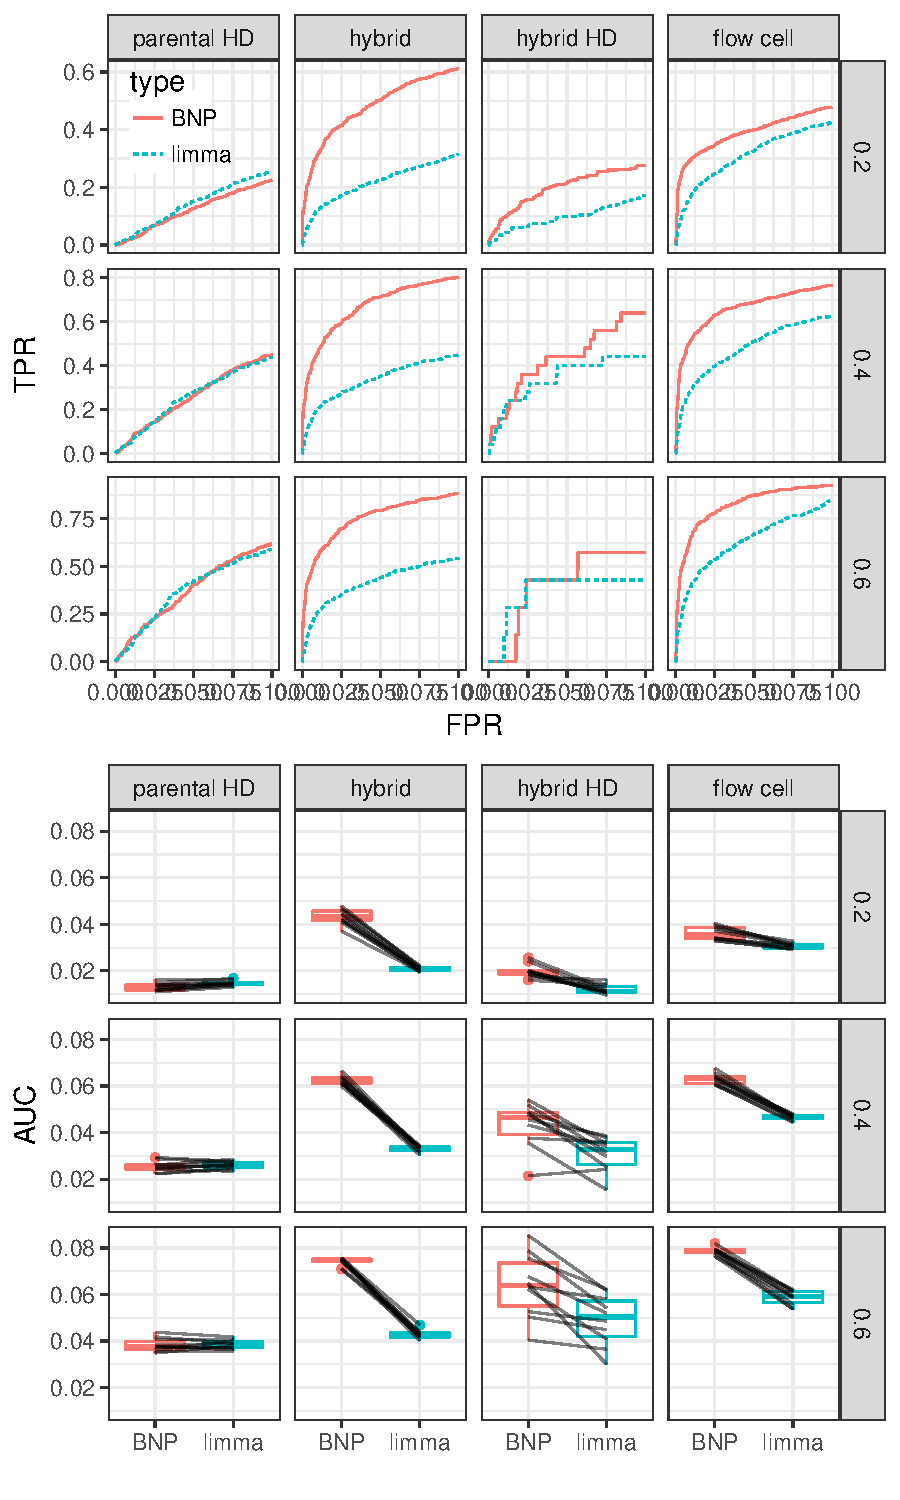
\includegraphics[height=.8\textheight]{ss1-roc-auc}
\begin{minipage}{.8\textwidth}
\caption{Comparison of gene classification accuracy for BNP and non-hierarchical log-linear model. \small Top: ROC curves for a typical simulated data set for classification of genes by whether or not a particular effect has a log-fold-change greater than a threshold. Bottom: Boxplots of AUC for the same tests for all ten simulations, up to a false discovery rate of 0.1. The black lines identify particular simulated data sets.}
\label{roc-ss1}
\end{minipage}
\end{figure}

\subsubsection{Precision of estimated effects}
We also compared the precision of point estimates obtained under the two models. For the BNP model, we take the posterior mean as our point estimate for $\beta_{g\ell}$. Here we expect BNP to do much better than limma because limma does not use a hierarchical model for shrinkage, whereas the BNP provides shrinkage toward the mass of the underlying distribution of the $\beta_g$s. Figure \ref{mspe-ss1} shows that this is indeed the case; the mean squared prediction errors averaging across genes are uniformly smaller that those for limma.

\begin{figure}[ht!]
\centering
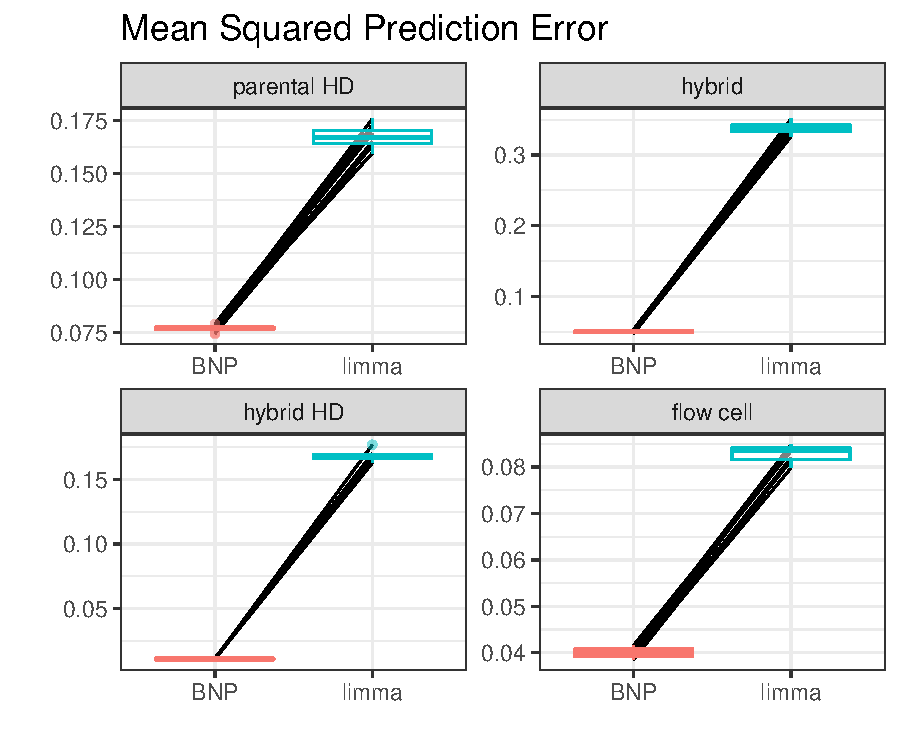
\includegraphics[width=.8\textwidth]{ss1-mspe}
\begin{minipage}{.8\textwidth}
\caption{\small Comparison of precision of coefficient estimation for BNP and non-hierarchical log-linear model. Mean squared prediction error for $\beta_{g\ell}$ averaging over $g$.}
\label{mspe-ss1}
\end{minipage}
\end{figure}

\subsection{Comparisons to count-based methods}
\label{sec:ss2}
Much of the recent methods proposed for the analysis of RNA-seq data are based on negative binomial generalized linear models. The goal of the following simulation study was to compare performance of the BNP method using the voom weights to popular negative binomial-based methods. To generate the count data, we first analyzed the \citet{paschold} data with the voom-limma pipeline. Each simulated data set was generated by first sampling a random subset of 10,000 genes without replacement. Next, we simulated normal data, conditioning on the estimates obtained by limma for $\beta_g$, $\sigma^2_g$, as well as the precision weights, computed by the voom, corresponding to the selected genes. These simulated log-cpm values were then converted to log-counts, centering by $\log_2(\bar{R}_\cdot)-\log_2(10^6)$, where $\bar{R}_\cdot$ is the geometric mean of the estimated effective library sizes from the original data. Finally, these log-counts ($\log_2 r_{gn}$) were exponentiated and rounded to obtain the simulated counts, $r_{gn}$. For each simulated data set, we analyzed the data using our BNP method and also with two popular count-based methods, \texttt{edgeR} and \texttt{DESeq2}, the latter both with and without independent normal priors on the $\beta_g$ parameters. \citep{edger2010,deseq2014}. Just as in the previous study, we considered precision of point estimates and accuracy of gene classification. The steps described above are outlined below. For each simulated data set, a single MCMC chain was run for 50,000 iterations after 10,000 burn-in iterations. These were thinned to yield 2,000 samples for each gene-specific parameter and $\alpha$. Geweke diagnostics for the gene-specific parameters showed slight departures from normality with a handful of genes having z-scores greater than 5 in absolute value. For every simulation 99\% of genes for every component had an ESS greater than 400, but every simulation had at least one gene with an ESS less than 100 and one simulation had a parameter with an ESS less than 10.

\begin{enumerate}
\item Sample 10,000 indices, $g$, from $\{1,2,\ldots,36,000\}$ without replacement.
\item Set $\beta_g:= \hat{\beta}_{voom,~g},\; \sigma^2_g:= \hat{\sigma}^2_{voom,~g}$
\item Sample $y_{gn} \sim \op{N}(x_{n}^\top\beta_g, \sigma^2_g/w_{gn})$
\item Set $r_{gn} = \op{Round} \left\{ 2^{y_{gn} + \log_2(10^6) - \log_2(\bar{R}_{\cdot})} \right\}$
\end{enumerate}


% Ranking accuracy (ROCs)
\subsubsection{Classification accuracy}
The methodologies of \citet{edger2010} and \citet{deseq2014} implemented in the \texttt{R} packages,\texttt{edgeR} and \texttt{DESeq2}, both provide threshold tests analogous to TREAT in \texttt{limma}. \citet{deseq2014} provide the option of employing empirical Bayes priors to $\beta_g$; we show results both with (shrunk) and without (unshrunk). We again used ROC to compare the accuracy in gene ranking between these three methods. For this simulation, unlike the first, the true parameters for each gene are unique. 

Comparing AUC across the ten simulations (Figure \ref{ss2-roc}), we see that, in most cases, \texttt{DESeq2} provides better rankings without the empirical Bayes prior. The AUCs for the other three methods are comparable, with small differences depending on the effect type and the threshold. Overall, it appears that BNP and \texttt{DESeq2} (unshrunk) have an edge over edgeR and that BNP may have a slight advantage over the other methods when the threshold is set fairly high.

\begin{figure}[ht!]
\centering
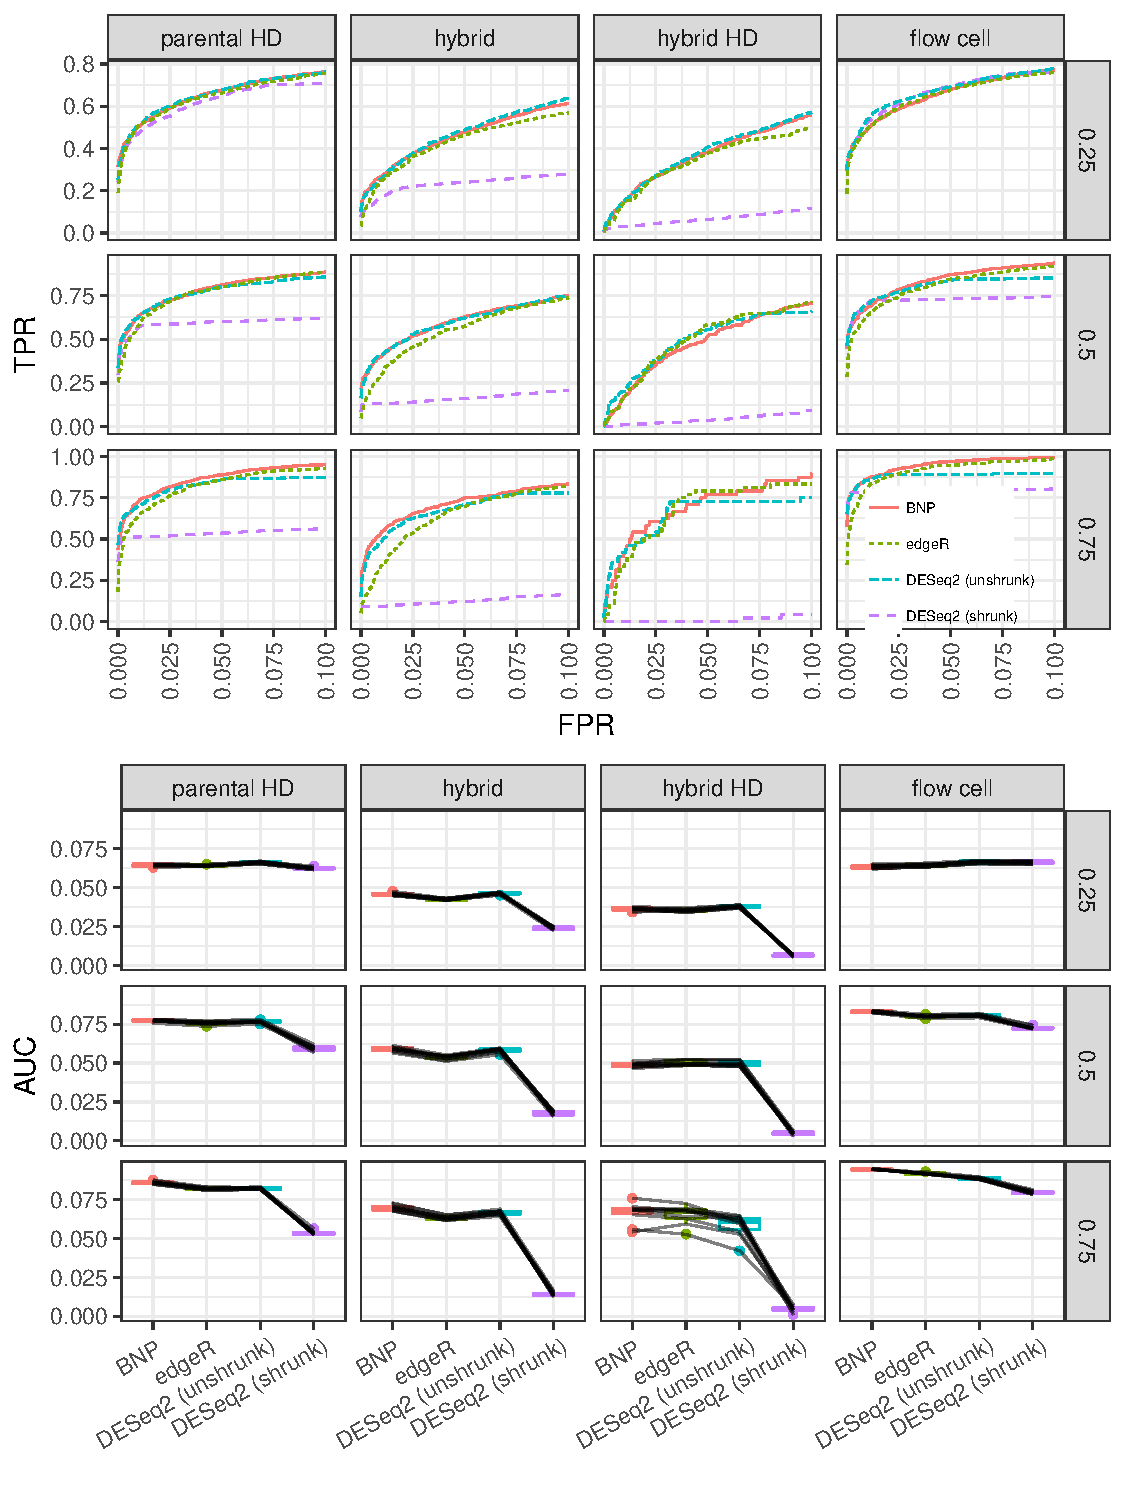
\includegraphics[height=.8\textheight]{ss2-roc-auc2}
\begin{minipage}{.8\textwidth}
\caption{\small Comparison of gene classification accuracy for BNP using voom weights and some popular count-based methods. \small Top: ROC curves for a typical simulated data set for classification of genes by whether or not a particular effect has a log-fold-change greater than a threshold. Bottom: Boxplots of AUC for the same tests for all ten simulations, up to a false discovery rate of 0.1. The black lines identify particular simulated data sets.}
\label{ss2-roc}
\end{minipage}
\end{figure}

\subsubsection{Precision of estimated effects}
% Mean squared prediction error
Plots of MSPE for the 10 simulations, shown in Figure \ref{ss2-mspe}, show that BNP compares favorably to the other methods, producing estimates that are closer to the truth, on average, that the count-based methods we tried. We expected that the empirical Bayes version of \texttt{DESeq2} would do better than the unshrunk version, since regularization of estimates typically reduces MSE. However, that was true only for the hybrid half-difference and the flow cell effect; for the parental half-difference and the hybrid effect, the unshrunk \texttt{DESeq2} estimates were more accurate.

\begin{figure}[ht!]
\centering
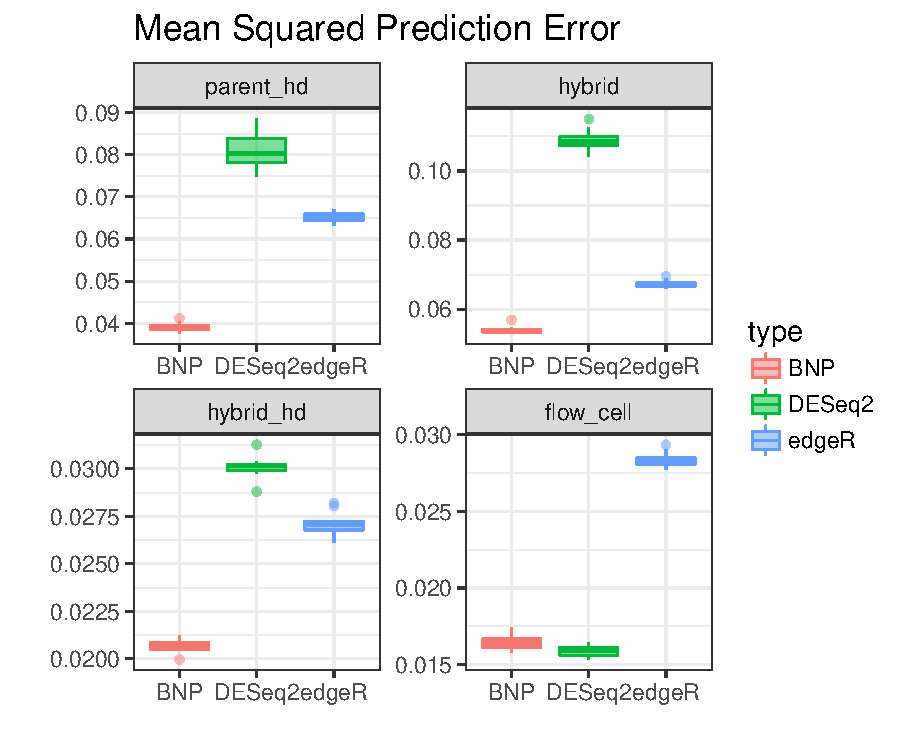
\includegraphics[width=.8\textwidth]{ss2-mspe}
\begin{minipage}{.8\textwidth}
\caption{\small Comparison of precision of coefficient estimation for BNP and non-hierarchical log-linear model. Mean squared prediction error for $\beta_{g\ell}$ averaging over $g$.}
\label{ss2-mspe}
\end{minipage}
\end{figure}

\subsection{Calibration of posterior probabilities}
Due to being fully Bayesian, the BNP method enjoys a further advantage over these other methods in that, by using posterior samples, we can evaluate probabilites of hypotheses with composite null parameter spaces which cannot be done using any of the other methods we tried. The ROC plots do suggest that the posterior probabilites do a good job with ranking the genes. However, because they are interpretable as probabilites, we can still question their accuracy relative to the frequency of true positives.

We now turn to four types of heterosis mentioned earlier in Section \ref{intro-paschold}. These are defined in terms of our parameterization of the model matrix in Table \ref{def-heterosis}.

Figure \ref{calib-ss2} shows estimated calibration curves for the 10 simulation studies for low- and high-parent heterosis for both of the two hybrid genotypes. Each curve was produced by binning genes by binning genes with similar posterior probabilites and plotting relative frequency of ``true-positives" vs. the midpoint probability of the bin. Ideally, these curves would follow the identity line. We don't view the deviations that we see as seriously compromising our approach, but we note that there do appear to be some biases. In particular, the sideways ``S" shape in the plot for low-parent B73$\times$Mo17, suggets that the posterior probabilities tend to be pulled away from moderate values for this particular hypothesis. 
%\citet{wang-phd} discussed how the geometry of the null parameter space for heterosis leads to serious difficulties with classical likelihood ratio tests; not the least of which is that p-values are not uniformly distributed under the null hypothesis, invalidating assumptions needed to apply corrections for multiple testing.

\begin{table}
\caption{Definition of types of gene heterosis in terms of mean expression by genotype as well as using parameterization implied by the design matrix.}
\label{def-heterosis}
\begin{tabular}{ccc}
Type of heterosis & Relation & $\beta$-parameterization\\
high-parent B73xMo17 & $\max\{\mbox{B73,Mo17}\} < \mbox{B73xMo17}$ & $\phantom{-}|\beta_{g2}| < \beta_{g3} + \beta_{g4}$\\
low-parent B73xMo17  & $\min\{\mbox{B73,Mo17}\} > \mbox{B73xMo17}$ & $-|\beta_{g2}| > \beta_{g3} + \beta_{g4}$\\
high-parent Mo17xB73 & $\max\{\mbox{B73,Mo17}\} < \mbox{Mo17xB73}$ & $\phantom{-}|\beta_{g2}| < \beta_{g3} - \beta_{g4}$\\
low-parent Mo17xB73  & $\min\{\mbox{B73,Mo17}\} > \mbox{Mo17xB73}$ & $-|\beta_{g2}| > \beta_{g3} - \beta_{g4}$
\end{tabular}
\end{table}



\begin{figure}[ht!]
\centering
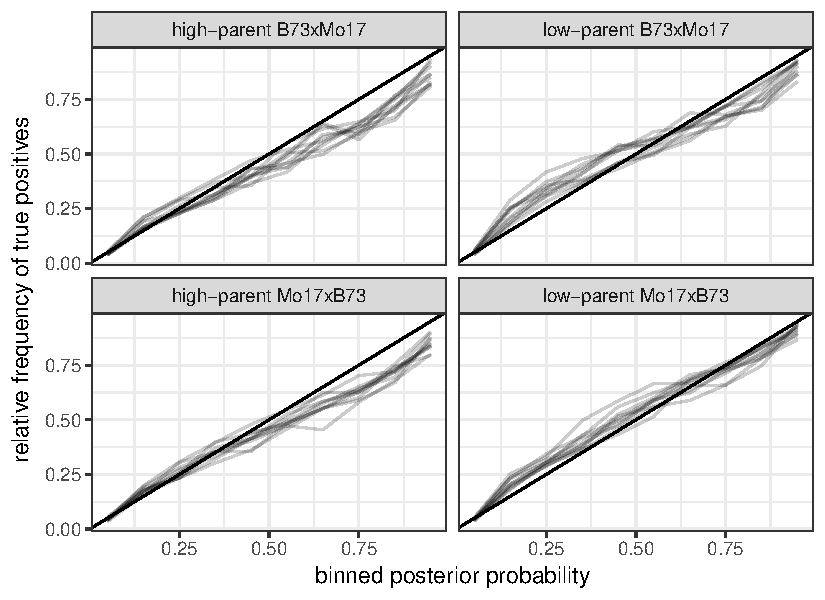
\includegraphics[width=.8\textwidth]{calib-ss2}
\begin{minipage}{.8\textwidth}
\caption{\small Calibration curves for BNP posterior probabilities calculated using posteriors and truth from the count-based simulations. Curves show true relative frequencies for the hypothesis indicated with bins determined by the posterior probability for each gene. The midpoint of the interval was used for plotting.}
\label{calib-ss2}
\end{minipage}
\end{figure}

\section{Analysis of Paschold data}
\label{analysis}
To fit the Paschold data, we ran 4 chains, each for 40,000 iterations after 30,000 iterations of warmup. The samples were thinned by a factor of 40, for a total of 160,000 post burn-in draws (4,000 thinned post burn-in draws) for each gene-specific parameter and $\alpha$. Posterior probabilities of the four heterosis hypotheses as well as posterior first- and second-moments for the gene-specific parameters, $\beta_g$ and $\sigma_g$, were computed using all the draws. Potential scale reduction factors were calculated for all of the gene-specific parameters and $\alpha$. Rhats for all parameters were less than 1.1.

\subsection{Comparison to original results}

In \citet{paschold}, the results of a series of hypothesis tests were combined to classify genes into several categories characterizing an ordering or partial ordering of the low-parent, high-parent and hybrid expression levels \citep[p.2448]{paschold}. LPH and HPH each correspond to a union of 2 of these categories ($\{7,8\}$ and $\{5,6\}$, respectively.) In Figure \ref{orig-compare}, we show histograms of posterior probabilities pertaining to high- and ow-parent gene heterosis for the genes subsetted by whether or not they were classified as ``discoveries'' in the original paper. High-parent heterosis corresponds to genes for which the mean expression of the hybrid is higher than the more highly expressed parent and low-parent heterosis where it is lower than the less expressed parent. Generally speaking, the posterior probabilities tend to agree with the categorization --- particularly for non-discoveries --- however, a number of discoveries have low posterior probabilities in our analysis. This is likely due to borrowing of information across genes leading to shrinkage toward general patterns of expression, where both low- and high- parental expression were uncommon (\citet{paschold} found evidence of these extreme patterns in less than 1\% of genes.) We also note that a small number of non-discoveries are found to have high-posterior heterosis probabilities. Due to the multidimensional shrinkage featured by the model, it can be difficult to sort out what accounts for the difference in some cases.

\begin{figure}[h!]
\centering
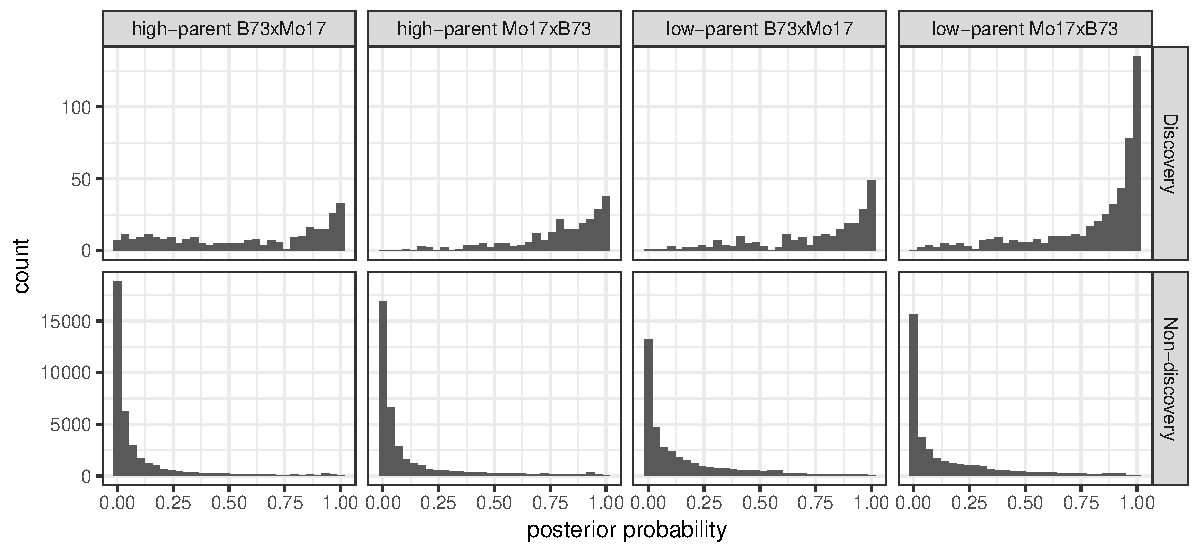
\includegraphics[width=\textwidth]{orig-compare}
\begin{minipage}{.8\textwidth}
\caption{\small Posterior probabilities for low- and high-parent gene heterosis hypotheses for subsets of genes classified as discoveries and non-discoveries in the original paper (Paschold et al. 2012).}
\label{orig-compare}
\end{minipage}
\end{figure}

Figure \ref{het-shrink} shows how the nonparametric model shrinks estimates. Genes categorized as showing evidence of extreme gene heterosis in the original paper are represented as black points. The left panel shows independently obtained estimates for the parental half-difference and the mean hybrid effect overlayed on a bivariate histogram of the independent estimates for all genes. The right
panel shows the corresponding estimates for our analysis overlayed on a posterior pointwise estimate of $\mathcal{P}$. In this second plot we can see significant shrinkage toward the regions where $\mathcal{P}$ has higher posterior density. This helps to explain why a large number of discovered genes have low posterior probabilities for the heterosis hypotheses: when weighed against the overall patterns within the data, in many cases it is likely that the magnitude of the independent estimates is overstated and that detection was a result of random variation.

A result of this shrinkage is increased posterior precision. Figure \ref{exemplars} shows 90\% posterior credible intervals for the exemplar genes from Table \ref{counts}. The credible intervals are fairly tight, and the posterior means fall outside the range of the data in some cases. This is a result of shrinkage due to the borrowing of information.

\begin{figure}[ht!]
\centering
\includegraphics[width=.7\textwidth]{exemplars_v2}
\begin{minipage}{.8\textwidth}
\caption{\small Plots of the exemplar genes from Table \ref{counts}, illustrating presence and absence of patterns of heterosis. The points are jittered horizontally. The uncertainty intervals shown are 90\% credible intervals for the mean log-cpm, scaled to the counts per million scale.}
\label{exemplars}
\end{minipage}
\end{figure}

\subsection{Comparison of heterosis results to parametric analysis}

\citet{landau2016high} undertook an analysis of the same data. They modeled the counts directly with a Poisson distributions, using a generalized linear model with log link and gene-specific linear predictors as well as a gene-specific variance parameter for a lognormal mixture on the means. They also assumed a parametric distribution for the gene-specific parameters. Their hierarchical model assumed independent normal priors on the coefficient components, $\beta_{g\ell}$. Table \ref{bayes-compare1} shows a comparison of the posterior probabilities found by our method to Landau's binned into five intervals for each of the four types of extreme heterosis. While there is a fair amount of agreement between these two methods on the genes with highest and lowest probabilities of heterosis, the differences between the inferences are considerable.

% latex table generated in R 3.4.2 by xtable 1.8-2 package
% Tue Nov 14 21:58:47 2017
\begin{table}[ht]
\footnotesize
\centering
\caption{Two-way tables comparing the posterior probabilities of low-parent gene heterosis for all genes in the Paschold et al. (2012) data set found by BNP and Landau and Niemi (2016).}
\label{bayes-compare1}
% % \begin{tabular}{rrrrrr}
% % &  &\multicolumn{4}{c}{Landau}\\
% %   \toprule
% % & & [0,0.25] & (0.25,0.5] & (0.5,0.75] & (0.75,1] & total\\
% %   \midrule
% % \multirow{4}{*}{BNP} & [0,0.25] & 20435 & 5499 & 1687 & 702 \\
% %   & (0.25,0.5] & 1299 & 1978 & 930 & 550 \\
% %   & (0.5,0.75] & 446 & 1115 & 486 & 509 \\
% %   & (0.75,1] & 148 & 287 & 167 & 583 \\
% %   & total
% %    \bottomrule
\begin{tabular}{rrrrrrr|r}
&  &\multicolumn{6}{c}{Landau and Niemi (2016)}\\
  \toprule
&  & [0,0.05] & (0.05,0.15] & (0.15,0.85] & (0.85,0.95] & (0.95,1] & total \\
  \midrule
\multirow{6}{*}{BNP} & [0,0.05]    & 0.283 & 0.083 & 0.116 & 0.001 & 0.000 & 0.483 \\
                     & (0.05,0.15] & 0.017 & 0.037 & 0.129 & 0.003 & 0.001 & 0.186 \\
                     & (0.15,0.85] & 0.009 & 0.025 & 0.254 & 0.017 & 0.009 & 0.313 \\
                     & (0.85,0.95] & 0.000 & 0.000 & 0.007 & 0.002 & 0.002 & 0.011 \\
                     & (0.95,1]    & 0.000 & 0.000 & 0.003 & 0.001 & 0.003 & 0.007 \\
                     \midrule
                     & total       & 0.308 & 0.145 & 0.508 & 0.022 & 0.016 & 1.000 \\
   \bottomrule
\end{tabular}
\\[.5cm]
Low-parent heterosis B73$\times$Mo17.
\\[.75cm]

% \begin{tabular}{rrrrrr}
% &  &\multicolumn{4}{c}{Landau}\\
%   \toprule
% & & [0,0.25] & (0.25,0.5] & (0.5,0.75] & (0.75,1] \\
%   \hline
% \multirow{4}{*}{BNP} & [0,0.25] & 21486 & 4557 & 1486 & 677 \\
%  &  (0.25,0.5] & 1639 & 2155 & 611 & 306 \\
%  &  (0.5,0.75] & 301 & 989 & 522 & 390 \\
%  &  (0.75,1] & 140 & 677 & 197 & 688 \\
%    \bottomrule
   \begin{tabular}{rrrrrrr|r}
&  &\multicolumn{6}{c}{Landau and Niemi (2016)}\\
  \toprule
&  & [0,0.05] & (0.05,0.15] & (0.15,0.85] & (0.85,0.95] & (0.95,1] & total \\
  \midrule
\multirow{6}{*}{BNP} & [0,0.05] & 0.296 & 0.090 & 0.135 & 0.003 & 0.001 & 0.523 \\
                     & (0.05,0.15] & 0.021 & 0.036 & 0.093 & 0.002 & 0.001 & 0.152 \\
                     & (0.15,0.85] & 0.010 & 0.031 & 0.237 & 0.011 & 0.005 & 0.295 \\
                     & (0.85,0.95] & 0.000 & 0.000 & 0.015 & 0.002 & 0.003 & 0.021 \\
                     & (0.95,1] & 0.000 & 0.000 & 0.003 & 0.002 & 0.005 & 0.010 \\
                     \midrule
                     & total & 0.327 & 0.157 & 0.483 & 0.020 & 0.014 & 1.000 \\
   \bottomrule
\end{tabular}
\\[.5cm]
Low-parent heterosis Mo17$\times$B73.
\end{table}

\begin{table}[ht]
\footnotesize
\centering
\caption{Two-way tables comparing the posterior probabilities of high-parent heterosis for all genes in the Paschold et al. (2012) data set found by BNP and Landau and Niemi (2016).}
\label{bayes-compare2}
   \begin{tabular}{rrrrrrr|r}
&  &\multicolumn{6}{c}{Landau and Niemi (2016)}\\
  \toprule
&  & [0,0.05] & (0.05,0.15] & (0.15,0.85] & (0.85,0.95] & (0.95,1] & total \\
  \midrule
\multirow{6}{*}{BNP} & [0,0.05] & 0.395 & 0.126 & 0.155 & 0.000 & 0.000 & 0.676 \\
                     & (0.05,0.15] & 0.037 & 0.037 & 0.085 & 0.000 & 0.000 & 0.159 \\
                     & (0.15,0.85] & 0.020 & 0.025 & 0.100 & 0.003 & 0.001 & 0.149 \\
                     & (0.85,0.95] & 0.000 & 0.000 & 0.011 & 0.001 & 0.001 & 0.012 \\
                     & (0.95,1] & 0.000 & 0.000 & 0.003 & 0.001 & 0.001 & 0.005 \\
                     \midrule
                     & total & 0.452 & 0.187 & 0.353 & 0.005 & 0.002 & 1.000 \\
   \bottomrule
\end{tabular}
\\[.5cm]
High-parent heterosis B73$\times$Mo17.
\\[.75cm]

\begin{tabular}{rrrrrrr|r}
&  &\multicolumn{6}{c}{Landau and Niemi (2016)}\\
  \toprule
&  & [0,0.05] & (0.05,0.15] & (0.15,0.85] & (0.85,0.95] & (0.95,1] & total \\
  \midrule
\multirow{6}{*}{BNP} & [0,0.05] & 0.352 & 0.115 & 0.165 & 0.000 & 0.000 & 0.633 \\
                     & (0.05,0.15] & 0.035 & 0.032 & 0.087 & 0.000 & 0.000 & 0.155 \\
                     & (0.15,0.85] & 0.033 & 0.035 & 0.116 & 0.005 & 0.002 & 0.190 \\
                     & (0.85,0.95] & 0.001 & 0.001 & 0.014 & 0.001 & 0.001 & 0.017 \\
                     & (0.95,1] & 0.000 & 0.000 & 0.003 & 0.001 & 0.001 & 0.005 \\
                     \midrule
                     & total & 0.421 & 0.183 & 0.386 & 0.007 & 0.003 & 1.000 \\
   \bottomrule
\end{tabular}
\\[.5cm]
High-parent heterosis Mo17$\times$B73.
\end{table}


From the marginal distributions of probabilities, we see that BNP finds lower chances of LPH across genes than Landau. For example, Landau found 1.6\% of genes to have greater than 95\% probability of low-parent heterosis for B73$\times$Mo17, but the majority of these were given less than 85\% probability by BNP. However, BNP also found higher probabilities for some genes: More than 1/3 of the 0.7\% genes which BNP found to be high probablity genes ($>$95\%) were found to only have moderate probabilities (15\%-85\%). The story is different for HPH. Here, BNP has greater confidence, finding both more high- and low-probability genes than Landau.

While we cannot say from these comparisons whether one model is better than another, they serve to highlight the impact that distributional assumptions can have in detecting patterns of gene expression. Given our belief that models like that of \citet{landau2016high} and \citet{deseq2014} make unreasonable assumptions about the distribution of the gene-specific parameters, we expect that the BNP probabilites incorporate more information about the broader patterns of expression exhibited in the data.

\iftoggle{thesis}{
\subsection{Some practical considerations}
On a different note, \citet{landau2016high} found that when an independent normal model was assumed for $\beta_{gl}$, their posterior distributions were well approximated by a normal distribution matching the first two posterior moments. This is convenient because computation of these moments requires minimal storage, as running means can be used to update these after each iteration of the MCMC chain.

Figure \ref{compare-to-approx} shows full posterior distributions and normal approximations for each component of $\beta_g$ for four randomly selected genes. The quality of the moment-based approximation is satisfactory in some cases but not in others. Due to the discrepencies displayed here, we would recommend basing inference on the full posterior, rather than a normal approximation. %In our experience, multimodality in posterior plots such as Figure \ref{compare-to-approx} can be suggestive that the MCMC has not converged. However, 
The traceplots for these parameters (Figure \ref{mixing}) show no indication of a lack of convergence. %this to be the case; rather, we suspect this is a feature of the nonparametric model. 
For reference, the data and estimated mean expression levels are displayed in Figure \ref{compare-cis}.
%figures for 4 random genes
\begin{figure}[ht!]
\centering
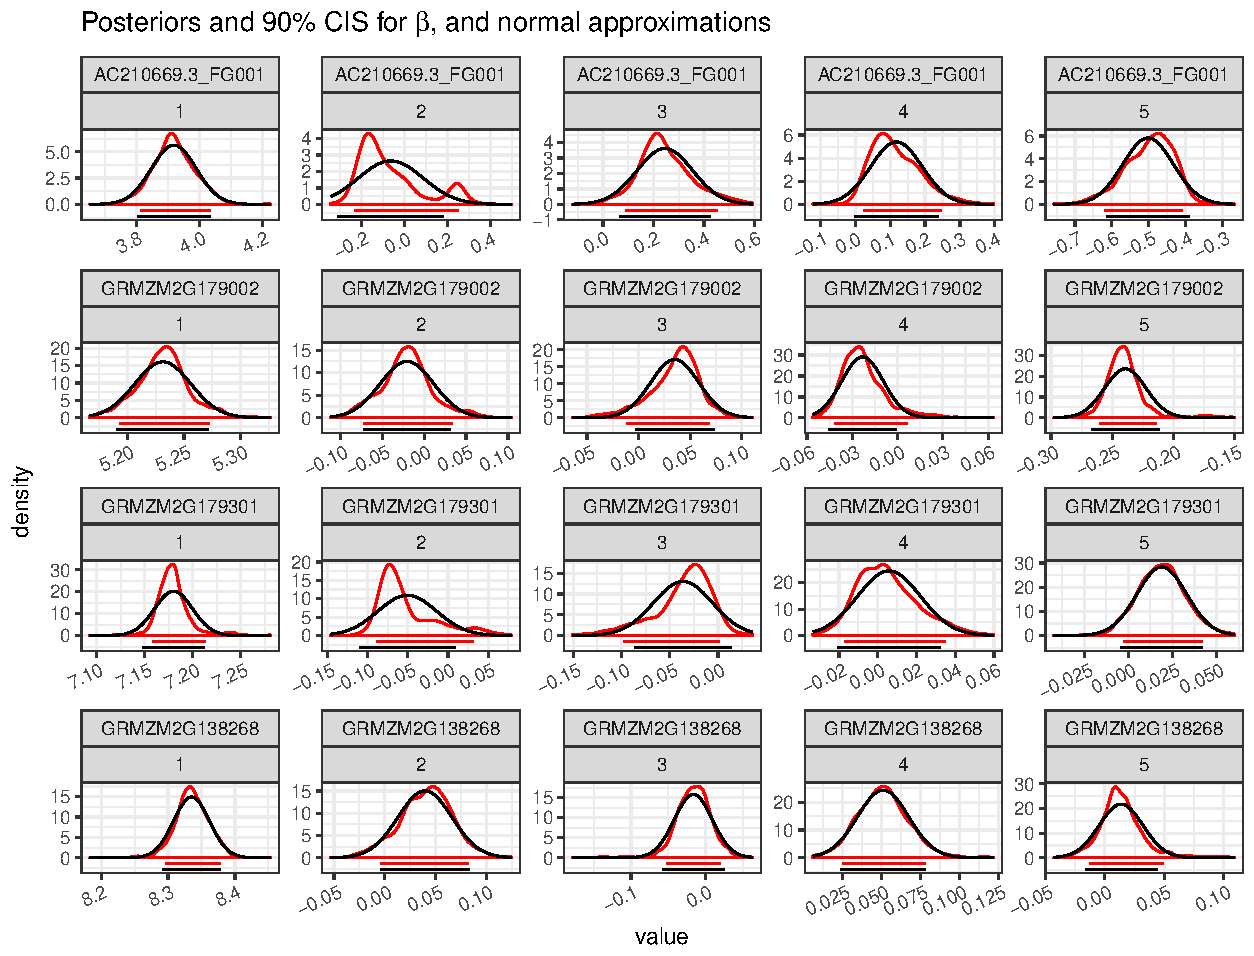
\includegraphics[width=\textwidth]{sample_genes_cis}
\begin{minipage}{.8\textwidth}
\caption{Posterior distributions of $\beta_g$ for 4 randomly selected genes (red). Normal approximations based on the first two posterior moments are also shown (black). Line segments representing 90\% credible intervals are drawn in the lower part of each plot. }
\label{compare-to-approx}
\end{minipage}
\end{figure}

\begin{figure}[ht!]
\centering
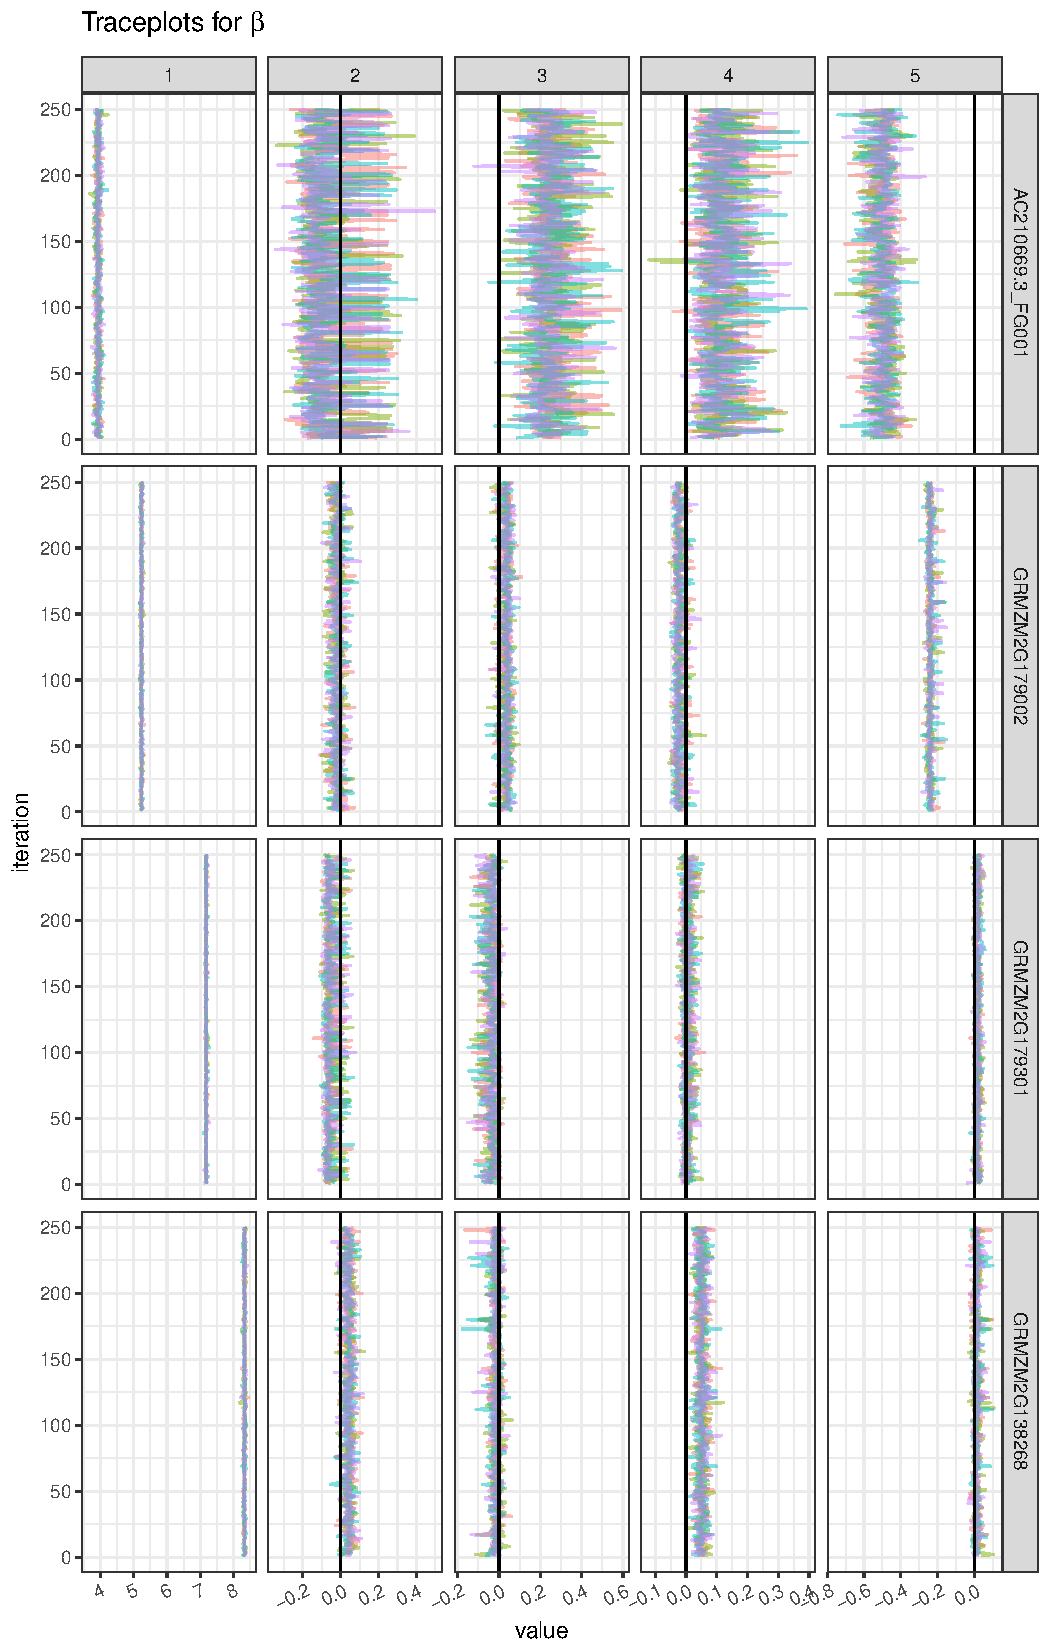
\includegraphics[width=.8\textwidth]{sample_genes_trace}
\begin{minipage}{.8\textwidth}
\caption{Traceplots of $\beta$ for randomly selected genes. 250 thinned samples for each independent Markov chain, the chain identified by color, are shown.}
\label{mixing}
\end{minipage}
\end{figure}

\begin{figure}[ht!]
\centering
\includegraphics[width=.7\textwidth]{sample_genes_mean_v2}
\begin{minipage}{.8\textwidth}
\caption{Adjusted log-cpm for randomly selected genes by genotype (black) and corresponding posterior means and 90\% confidence intervals for the mean log-cpm expression, transformed to the counts per million scale (red).}
\label{compare-cis}
\end{minipage}
\end{figure}
}




% Thresholding by $\mu_{12} - t > \max\left\{\mu_1,\mu_2\right\} \implies \beta_3+\beta_4 > |\beta_2|$

\begin{figure}[h!]
\centering
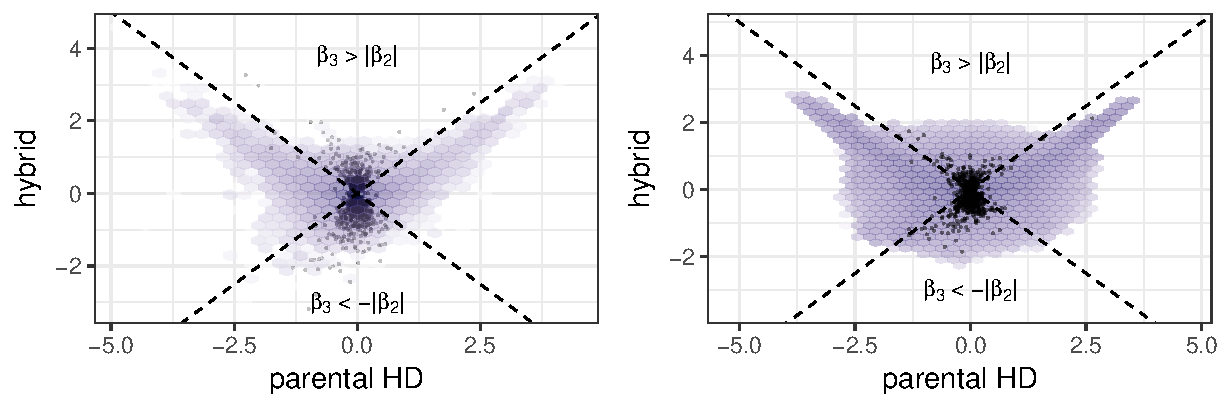
\includegraphics[width=\textwidth]{heterosis-shrinkage}
\begin{minipage}{.8\textwidth}
\caption{\small The left panel shows independently obtained estimates for the parental half-difference and the mean hybrid effect for genes classified as heterotic in the maize study. These are overlayed on a bivariate histogram of the independent estimates for all genes. The right
panel shows the corresponding estimates for our analysis overlayed on a posterior pointwise estimate of $\mathcal{P}$. In this second plot we can see significant shrinkage toward the regions where $\mathcal{P}$ puts more probability in the posterior.}
\label{het-shrink}
\end{minipage}
\end{figure}

\section{Discussion}
\label{sec:discussion}
Hierarchical models have an important role in problems where, as is true in gene expression, the number of model parameters is much larger than the number of subjects. By modeling the parameters, we use the ``between-gene" information in the data to moderate our inferences about individual genes . Where some methodolgies employ empirical Bayes concepts for certain procedures, hierarchical models are not usually an explicit part of the model. Empirical evidence suggests that, with regard to the gene-specific parameters, default model assumptions such as independent normals, are not realistic --- the empirical distributions exhibit irregular shapes, multimodality and correlations. Since it seems difficult to suggest a parametric alternative to the common default assumptions (independence, normality), a one-size-fits-all nonparametric model seemed worth investigating. We have demonstrated a computationally demanding, yet feasible, solution in our BNP method.

Our simulation studies show that the BNP methodology provides a viable alternative to more standard methods. Intuitively, we expect that it should do better than the alternative methods we considered in cases when the distribution of gene-effects has an unusual shape that contradicts independence. We can imagine situations where the underlying distribution of the gene specific parameters is itself an object of importance. For example, the v-shape displayed in Figure \ref{het-shrink} describes a pattern whereby the average hybrid mean expression tends toward but generally remains less than the mean expression of the higher parent. We might interpret this to be a result of dominance, where a dominant allele masks the effect of the recessesive allele in the heterozygous maize plant.

When there is only interest in expression at the level of genes, it should still be valuable to have a model flexible enough to handle detectable patterns in the data. Figure \ref{all-shrink} shows side-by-side plots of the distribution of the estimated components by BNP and \texttt{DESeq2}, which assumes independent priors on the gene-specific effects (excluding the intercept). The BNP estimates are shrunk toward the mass of the distribution, whereas \texttt{DESeq2} estimates are shrunk toward the origin.


\begin{landscape}
\begin{figure}
\centering
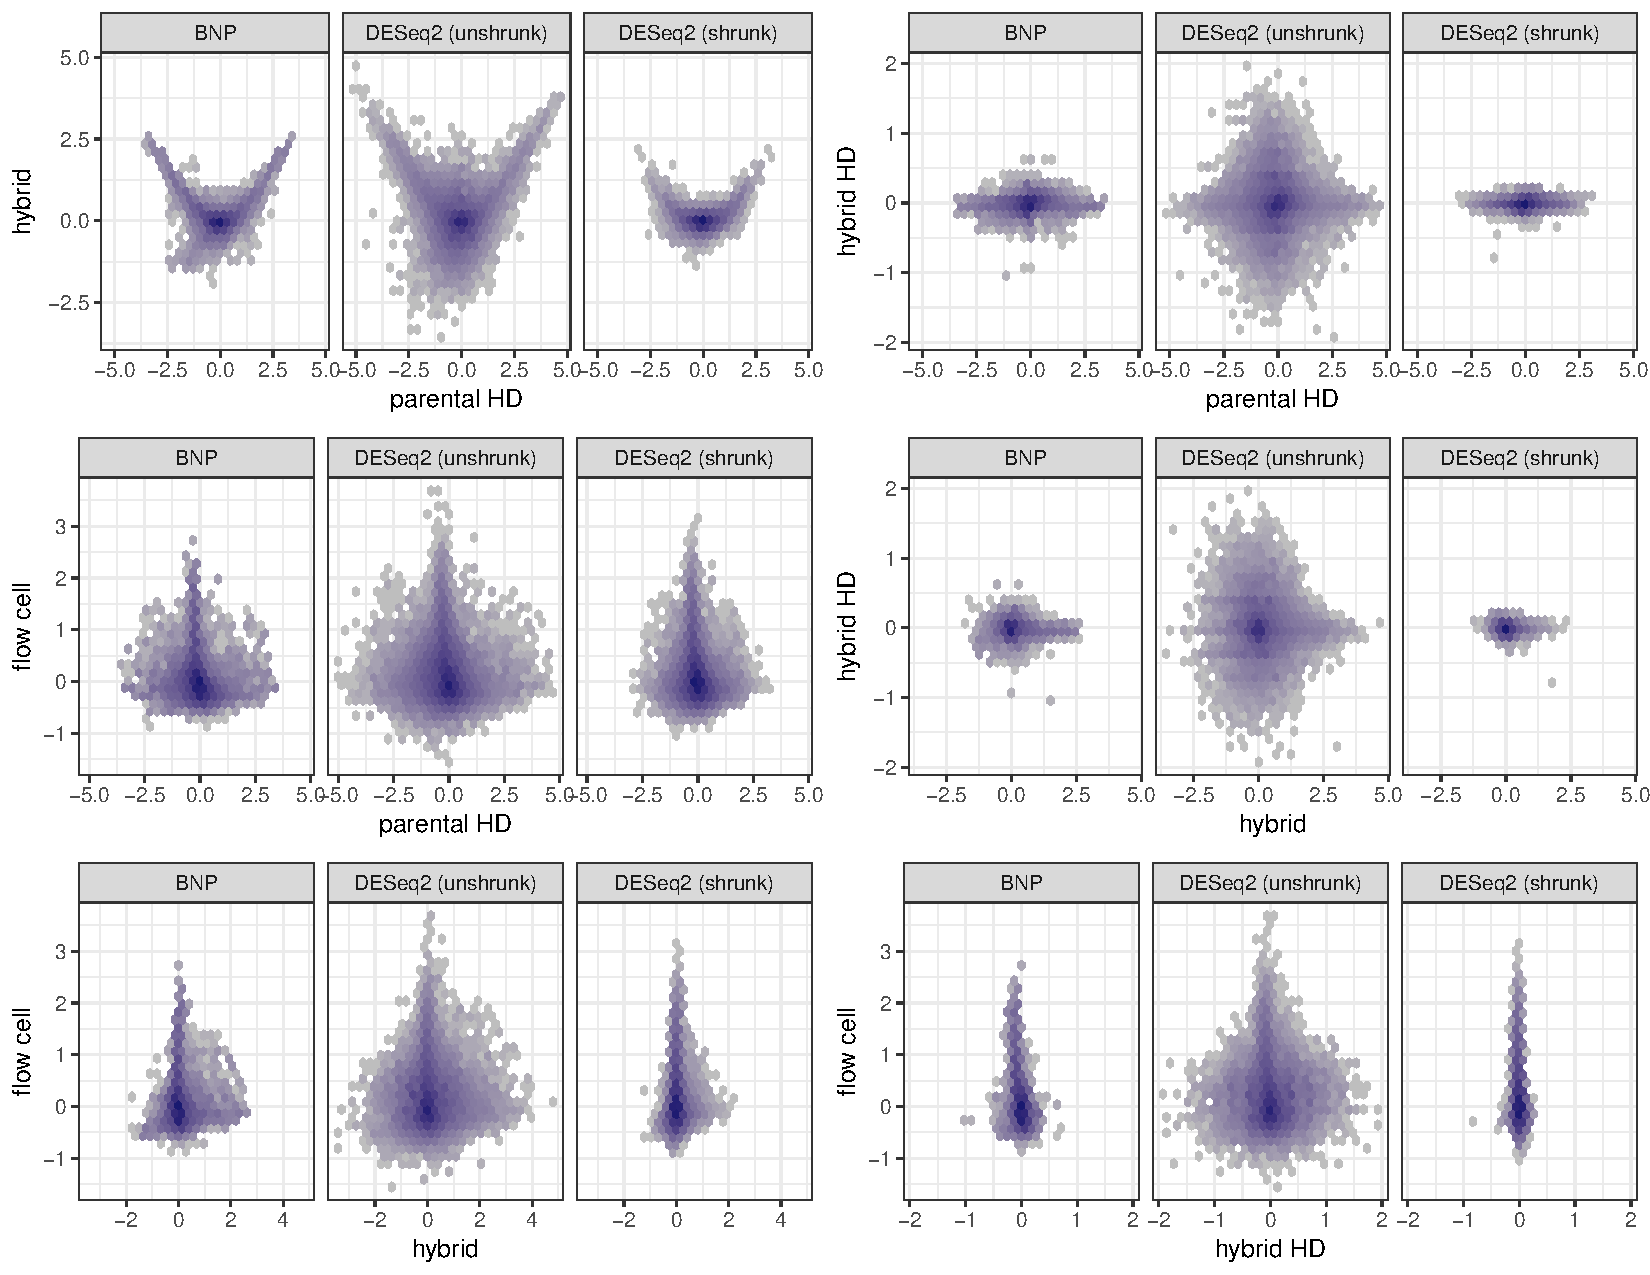
\includegraphics[height=.9\textheight]{pairs-shrinkage}
\caption{Bivariate histograms of estimates of gene-specific effects, excluding intercepts. The estimates shown are posterior means obtained with the BNP method as well as estimates obtained with DESeq2 with and without independent normal shrinkage priors (MAP and MLE, respectively) are shown.}
\label{all-shrink}
\end{figure}
\end{landscape}

Additionally, while posterior sampling is cumbersome in the amount of memory involved (approximately 6 GB for 4,000 samples of $\beta$), the interpretability of posterior quantities of interest and the inferential flexibility allowed make a strong case for the use of the Bayesian approach.



There are various modifications that might be considered to our model, within the same graphical structure. In the BNP method, precision weighting was used to correct for inaccuracies in mean-variance relationship implied by a normal assumption on the normalized log-counts. We would prefer not to have our inference conditional on these pre-computed estimates. An alternative approach would be to adopt an over-dispersed count model, such as the negative binomial and model the counts directly. Our reason for not doing this in the first place is that by proper choice of base measure, we get conditionally conjugate draws for $\tilde{\beta}_k$ and $\tilde{\sigma}^2_k$ that depend only on simple linear combinations of low-dimensional summaries of the counts. In contrast, the log-likelihood for the negative binomial involves quantities such as $\sum_n \log \Gamma(y_{gn}+\phi)$, for real-valued overdispersion parameter $\phi$, which is not linear in the parameter. Despite such nuisances, the overall structure of our Gibbs sampler would remain unchanged.

Another modification that we might consider is the choice of prior for the stick-breaking weights. The implication of the $\op{Beta}(1, \alpha)$ priors is that the weights decay exponentially on average. A generalization described in \cite{ishwaran2001} is $\nu \sim \op{Beta}(1-a, b + ak)$, which the authors refer to as a Pitman-Yor process, contains the Dirichlet process as a special case ($a=0,b=\alpha$). Other restrictions can selected to represent alternative prior assumptions. For example, one can select $a=\alpha, b=0$ which implies that the weights follow a power law. We might expect that this would lead to more significant weights and thus less aggressive shrinkage that the Dirichlet process.





\bigskip
\begin{center}
{\large\bf SUPPLEMENTARY MATERIAL}
\end{center}

\begin{description}

\item[Title:] Brief description. (file type)

\item[R-package for  MYNEW routine:] R-package ?MYNEW? containing code to perform the diagnostic methods described in the article. The package also contains all datasets used as examples in the article. (GNU zipped tar file)

\item[HIV data set:] Data set used in the illustration of MYNEW method in Section~ 3.2. (.txt file)

\end{description}


\bibliographystyle{plainnat}

\bibliography{methods}
\end{document}
